\documentclass[bachelor,openright,notchinese]{sustcthesis}
% 默认twoside 双面打印
% 将master修改为bachelor, doctor or master
% 要使用adobe字体,添加adobefonts选项
% 使用euler数学字体,如不愿使用,去掉euler
% 使用外文写作,请添加notchinese

% 设置图形文件的搜索路径
\graphicspath{{figures/}}



%%%%%%%%%%%%%%%%%%%%%%%%%%%%%%
%% 封面部分
%%%%%%%%%%%%%%%%%%%%%%%%%%%%%%



 % 中文封面内容
  \title{六次循环域}%一般情况下扉页和封皮、书脊共用一个标题文本,可以不用定义\spinetitle(仅硕博有用), \covertitle(本硕博均有用)和\encovertitle(仅本科有用)。特殊情况见下。
  %特殊情况1:本例中\title命令里含有换行控制字符,这会导致制作书脊的时候出现错误,例如如果你注释掉\spinetitle{...}这一行就会报错。这时需要定义一个不含换行等命令的\spinetitle,这并不表示\spinetitle里不能有任何命令——只能使用有限的命令。
  %特殊情况2:本例中标题过长,所以需要缩小书脊标题的字号。
  %特殊情况3:本例中中英文混排,由于tex竖排的原理限制,中英文基线不重合,所以需要人工调整英文的基线。具体调整量根据不同字体有所不同。
  %\covertitle{六次循环域}
  %\covertitle{中文题目第一行\\中文题目第二行}
  %不要在此调整封皮字体大小! Do not set Cover Page font size here!
  %特殊情况4:本例中\title中含有多个换行,导致标题超过了两行。根据制本厂规定,封皮标题不能超过两行。因此需要定义封皮使用的标题\covertitle. 如果你注释掉这一行,就会发现封皮不符合规定。
  %\encovertitle{On Cyclic Sextic Fields}
  %\encovertitle{English Title Line 1\\English Title Line 2\\English Title Line 3}
  %不要在此调整封皮字体大小! Do not set Cover Page font size here!
  %特殊情况5:仅本科生有用。本科封皮中有英文标题,不超过三行。与上类似。
  \author{张 \ 文 \ 超}
  \depart{金融数学系}%系别,硕博请用系代号,本科请用全称如
  \major{数学专业}%专业,硕博请用全称,本科不需要
  \advisor{李景治\ 教授}
  \coadvisor{张贤科\ 教授,\ 余解台\ 教授}%第二导师,没有请注释掉
  \studentid{11110015}%For bachelor only
  \submitdate{二〇一四年九月}

  % 英文封面内容
  \entitle{A FOG-BASED VIDEO DISTRIBUTION AND ACCESS NETWORK (Fog VDN)}
  \enauthor{Jiang. Yinghao}
  \studentid{11410423}
  \endepart{Computer Science and Engineering}
  \enmajor{Computer Science and Techonology}
  \enadvisor{ZHANG Jin}
%  \encoadvisor{Xianke Zhang(Number Theory)}
%  \encoadvisorsec{Jietai Yu(Galois Theory)}
  \ensubmitdate{June, 2018}

\begin{document}

% 封面
\maketitle

%特别注意,以下述顺序为准,在对应部分添加文档部件,切勿颠倒顺序:
%本科论文的文档部件顺序是:
%    frontmatter:致谢、目录、中文摘要、英文摘要、
%    mainmatter: 正文章节
%    backmatter: 参考文献或资料注释、附录
%%%%%%%%%%%%%%%%%%%%%%%%%%%%%%
%% 前言部分
%%%%%%%%%%%%%%%%%%%%%%%%%%%%%%
\frontmatter
\makeatletter

\ifustc@bachelor
	%%%%%%%%%%%%%%%%%
	%本科论文修改这里
	%%%%%%%%%%%%%%%%%
	% 致谢
	\chapter*{COMMITMENT OF HONESTY}
\label{chap:honest}

\begin{enumerate}
\item I solemnly promise that the paper presented comes from my
independent research work under my supervisor’s supervision. All
statistics and images are real and reliable.

\item Except for the annotated reference, the paper contents no other
published work or achievement by person or group. All people making
important contributions to the study of the paper have been indicated
clearly in the paper.
\item I promise that I did not plagiarize other people’s research achievement
or forge related data in the process of designing topic and research
content.

\item If there is violation of any intellectual property right, I will take legal
responsibility myself.
\end{enumerate}

\vskip 3\baselineskip


\begin{flushright}

Signature: \underline{\hspace{5cm}}
\vskip \baselineskip
Date :  \underline{\hspace{5cm}}

\end{flushright}

%	\chapter{Preface}
\label{chap:chap-preface}
This thesis is intended to summarize the learning outcomes and some works done by me during the undergraduate period in south university of science and technology of china (SUSTC). In this thesis, I choose two topics, one is related to algebraic number theory and the other one is something about function fields. The central idea or tool is the Galois theory, which connects the two part for this paper. For the number fields part, I have rearrange many references and books in order to give a simple and clear skeleton. For the function fields, we prove an explicit theorem, which is useful for studying the discrete (finite) subgroups of the automorphism group of a function field.  

Before the main contents of the thesis, I would like to take some words for my process on studying mathematics during the time in SUSTC. Although there is no mathematics department for our newly established university, I am grateful that I have learn many mathematics, especially abstract algebra, algebraic number theory and algebraic geometry from Prof. Xianke Zhang, and  Prof. Jietai Yu in the University of Hongkong etc.

As a student who loves mathematics very well, I have met so many kindly and responsible mathematicians during my 3.5-years' college life. During the first two years, as the 
representative of mathematics lessons in our inaugural class across all majors, I have ``obligation" to get good grades on mathematics lessons in order to set a good example. I learned Calculus and Analysis from Prof. Xuefeng Wang in mathematics department of Tulane University, Prof. Jinzhong Zhang in Guangzhou University, Prof. Zhongkan Liu in SUSTC and Beihang University, who is my first supervisor. We had frequent discussions on some topics on analysis as well as many other topics like elementary geometry and ordinary differential equation etc. 

After entering financial mathematics department, I also learned ordinary differential equation, probability, stochastic process, numerical methods, as well as some statistics from the professors in the department. Among of them, Prof. Anyue Chen, Prof. Jingzhi Li, Prof. Xuejun Jiang, Prof. Huaiqing Wang, Prof. Dejun Xie and Prof. Bianxia Sun gave me so many supports. Especially, Prof. Li, as my graduation designation supervisor, encouraged me a lot on studying algebra, and helped me to know some good mathematician friends of him.

Prof. Xianke Zhang, supervisor of me (after Prof. Liu) and an academic supervisor of this thesis, has guided me into the world of abstract algebra, a field which is quite abstruse for freshman. However, I found appealing thing inside the abstract definitions and complex relations one day. After that, besides the formal classes, we held several seminars on algebraic number theory and commutative algebra etc under the guidances of Prof. Zhang. 

Prof. Jietai Yu who has inspired me on Galois theory and algebraic geometry, has given me many guidances on research area as well as daily life. He gave us Galois courses as well as seminar on algebraic geometry. Among that time, I had my first opportunity to give a presentation in the formal seminar. I still remember the topics for that seminar is the finite subgroups of $\operatorname{PGL}(2,\mathbb{C})$ (we will show the relevant topic in chapter \ref{chap:chap-eight}). What's more, Prof. Yu found more opportunities for me to learn more mathematics as well as to further my study.

During those experiences outside the campus, I have learnt more recent works on affine algebraic geometry. The happiest things for me during those academic activities are finding many good friends, like Swapnil Lokhande, Sagar Kolte, Shameek Paul, Shihong Ma, Ju Huang, Haifeng Tian etc. They really gave me so much encouragement and concern. Also, I also met many good mathematician, like Prof. Alexey Belov, Prof. Leniod Makar-Limanov, Prof. Wenhua Zhao, Prof. Fang Li, Prof. Xiankun Du and so on. They gave me some instructions on some problems and encouraged me on studying mathematics.

Last but not least, I've come to realize that the ability of self-study is the most important good properties for a university student. I have paid much time to learn something outside the courses, to find some interesting topics, to sort out learning knowledge. During these years, I wrote a personal mathematics blog to record those things.


\vskip 28pt

\begin{flushright}

Wenchao ZHANG

September, 2014 at SUSTC

\end{flushright}






     


	%目录部分
	%目录
	\tableofcontents
	%默认表格、插图、算法索引名称分别为“表格索引”、“插图索引”和“算法索引”
	%如果需要自行修改lot,lof,loa的名称,请定义
	%\ustclotname{...}
	%\ustclofname{...}
	%\ustcloaname{...}

	% 表格索引
	%\ustclot
	% 插图索引
	%\ustclof
	%算法索引
	%如果需要使用算法环境并列出算法索引,请加入补充宏包。
	%\ustcloa

	% 摘要
	\begin{cnabstract}
近年来,人们对于视频(点播、直播)需求激增,寻找一个成本更低,用户体验更优,满足不断增长的视频播放需求
的视频内容分发系统迫在眉睫。雾节点(路由器,网络附加存储,智能家庭中心等)有着大量闲置的带宽、
存储、计算资源,可以很好的利用这些闲置资源来承担视频分发的功能。
然而,传统的内容分发网络系统以及点对点传输系统
并不能很好的应用于由数百万雾节点构成的新网络。

本论文中,我们给出了雾计算及其相关领域最新的研究应用进展综述。我们将雾节点构成的网络抽象为一个统一的模型,并且给出了关键
问题的解决方案。对于我们的算法、协议和架构也进行了讨论。

我们实现的是一个基于雾节点的视频分发系统,其中每个雾节点可以存储一些视频文件,当用户请求播放视频时,存有这些视频的
雾节点就相当于传统架构中的服务器。用户的随机请求分布符合视频的热度分布。我们的问题可以抽象为如何将视频分发到雾节点上
并且当用户进行视频播放时,在不影响用户体验的前提下,可以让云服务器的负载最小。

类似于我们讨论的问题的研究已经有了一些结论。本文首先对视频流行特征进行了概述,并对设计这样一个系统的基本原则进行了探讨,
并且展示了相关系统的最新研究进展。我们还提出并实现了一种简单的(初级版本)基于雾节点的分布式系统架构,
取得了一些测试数据,并对数据进行了分析研究,并尝试根据分析结果进行一些优化。

最后,我们试图找出一些系统的一些短板,并尝试推断我们未来可以从哪一些方面进行系统的优化。

\keywords{雾计算,内容分发网络(CDN),视频,信息中心网络(ICN),命名数据网络(NDN)}
\end{cnabstract}

\begin{enabstract}
With users rapid-growing demand on Video, including "Video-on-demand"(VoD) and Live Streaming and
its "Quality of Experience"(QoE), video service providers are facing new challenges and topics, those are,
to provide efficient video content transmission and easy network accessing procedure and application.
 Under the circumstance, the fog devices(Wi-Fi routers, Network Attached Storage and Smart home center)
 which have better bandwidth, storage and computation capacities, have come into the spotlight.
 Fog devices can collaboratively serve the local users by providing a new paradigm for video distribution.
  However, to coordinately manage millions of fog devices requires  new schemes that are different from
  both the traditional "Content Delivery Network"(CDN) and the Peer-to-Peer(P2P) schemes.

In this thesis, firstly, we provide an overview of recent research achievement in fog computing and related fields over the past two decades. We generalize the network which composed of fog nodes to a unified mode and give solutions to key problems. Algorithmic, protocol and architectural design principles are also discussed in this section.
 
Then we discuss a fog-based video distribution and access system where each fog nodes can store relatively small number of videos to offload the server when these videos are requested by users. Users’ stochastic requests are predictable based on videos popularity distribution pattern. The problem here is how to distribute the videos to the fog nodes and how to guide the users to get the video from these fog nodes to minimize the server load as well as to obtain a better user experience.
 
Similar issues have been studied recently witsome conclusion being reached to. In this thesis, We first overview the video popularity characteristics and discuss the fundamental challenges to design an effective fog-based video service platform and show the recent achievement on
some different video distribution and access systems. We also propose a simple(primarily) fog-based distribution and access system architecture, examine its capacities and try to do some optimization.
 
Finally, We try to figure out some related system defects and predict in which way could we optimize the system and make it better.

\enkeywords{Fog computing,Content Delivery Network(CDN), Video,Information Centric Networking(ICN),Named Data Networking (NDN)}
\end{enabstract}
%此文件中含有中英文摘要
   % \begin{denotation}
\item[$\mathbb{Q}$] rational number field
\item[$\mathbb{Z}$] rational integer ring
\item[$K$] algebraic number field
\item[$O_K$] the ring of integers of $K$
\item[$\operatorname{Aut}(K/F)$] Automorphism group of $K$ which fixes $F$
\item[$\operatorname{Gal}(K/F)$] Galois group of $K$ which fixes $F$
\item[$\operatorname{Res}(f,g)$] resultant of polynomials $f(x)$ and $g(x)$
\item[$R_{p,f}$] resolvent polynomial of $f(x)$ with $orb(p)$
\item[$\operatorname{Disc}(f)$] discriminant of polynomial $f$
\item[$\operatorname{Disc}(\theta)$] discriminant of minimal polynomial of $\theta$,i.e. $\operatorname{Disc}(1,\theta,\dots,\theta^{n-1})$
\item[$\operatorname{ht}(f)$] height (or degree) of a rational function $f$
\item[$d(K)$] discriminant of field $K$
\item[$\operatorname{N}(\alpha)$] Norm of $\alpha$
\item[$\operatorname{Tr}(\alpha)$] Trace of $\alpha$
\item[$C_n$] cyclic group
\item[$Cl(K)$] class group of $K$
\item[$h(K)$] class number of $K$
\item[$U(K)$] group of units in $K$
\item[$\zeta_n$] $n^{th}$ root of unity

\end{denotation}


\else
	%%%%%%%%%%%%%%%%%
	%硕博论文修改这里
	%%%%%%%%%%%%%%%%%
	% 摘要
	\begin{cnabstract}
近年来,人们对于视频(点播、直播)需求激增,寻找一个成本更低,用户体验更优,满足不断增长的视频播放需求
的视频内容分发系统迫在眉睫。雾节点(路由器,网络附加存储,智能家庭中心等)有着大量闲置的带宽、
存储、计算资源,可以很好的利用这些闲置资源来承担视频分发的功能。
然而,传统的内容分发网络系统以及点对点传输系统
并不能很好的应用于由数百万雾节点构成的新网络。

本论文中,我们给出了雾计算及其相关领域最新的研究应用进展综述。我们将雾节点构成的网络抽象为一个统一的模型,并且给出了关键
问题的解决方案。对于我们的算法、协议和架构也进行了讨论。

我们实现的是一个基于雾节点的视频分发系统,其中每个雾节点可以存储一些视频文件,当用户请求播放视频时,存有这些视频的
雾节点就相当于传统架构中的服务器。用户的随机请求分布符合视频的热度分布。我们的问题可以抽象为如何将视频分发到雾节点上
并且当用户进行视频播放时,在不影响用户体验的前提下,可以让云服务器的负载最小。

类似于我们讨论的问题的研究已经有了一些结论。本文首先对视频流行特征进行了概述,并对设计这样一个系统的基本原则进行了探讨,
并且展示了相关系统的最新研究进展。我们还提出并实现了一种简单的(初级版本)基于雾节点的分布式系统架构,
取得了一些测试数据,并对数据进行了分析研究,并尝试根据分析结果进行一些优化。

最后,我们试图找出一些系统的一些短板,并尝试推断我们未来可以从哪一些方面进行系统的优化。

\keywords{雾计算,内容分发网络(CDN),视频,信息中心网络(ICN),命名数据网络(NDN)}
\end{cnabstract}

\begin{enabstract}
With users rapid-growing demand on Video, including "Video-on-demand"(VoD) and Live Streaming and
its "Quality of Experience"(QoE), video service providers are facing new challenges and topics, those are,
to provide efficient video content transmission and easy network accessing procedure and application.
 Under the circumstance, the fog devices(Wi-Fi routers, Network Attached Storage and Smart home center)
 which have better bandwidth, storage and computation capacities, have come into the spotlight.
 Fog devices can collaboratively serve the local users by providing a new paradigm for video distribution.
  However, to coordinately manage millions of fog devices requires  new schemes that are different from
  both the traditional "Content Delivery Network"(CDN) and the Peer-to-Peer(P2P) schemes.

In this thesis, firstly, we provide an overview of recent research achievement in fog computing and related fields over the past two decades. We generalize the network which composed of fog nodes to a unified mode and give solutions to key problems. Algorithmic, protocol and architectural design principles are also discussed in this section.
 
Then we discuss a fog-based video distribution and access system where each fog nodes can store relatively small number of videos to offload the server when these videos are requested by users. Users’ stochastic requests are predictable based on videos popularity distribution pattern. The problem here is how to distribute the videos to the fog nodes and how to guide the users to get the video from these fog nodes to minimize the server load as well as to obtain a better user experience.
 
Similar issues have been studied recently witsome conclusion being reached to. In this thesis, We first overview the video popularity characteristics and discuss the fundamental challenges to design an effective fog-based video service platform and show the recent achievement on
some different video distribution and access systems. We also propose a simple(primarily) fog-based distribution and access system architecture, examine its capacities and try to do some optimization.
 
Finally, We try to figure out some related system defects and predict in which way could we optimize the system and make it better.

\enkeywords{Fog computing,Content Delivery Network(CDN), Video,Information Centric Networking(ICN),Named Data Networking (NDN)}
\end{enabstract}
%此文件中含有中英文摘要
	% 目录
	\tableofcontents
	%默认表格、插图、算法索引名称分别为“表格索引”、“插图索引”和“算法索引”
	%如果需要自行修改lot,lof,loa的名称,请定义
	%\ustclotname{...}
	%\ustclofname{...}
	%\ustcloaname{...}

	% 表格索引
	\ustclot
	% 插图索引
	\ustclof
	%算法索引
	%如果需要使用算法环境并列出算法索引,请加入补充宏包。
	%\ustcloa

	%符号说明,需要加入补充包
%	\begin{denotation}
\item[$\mathbb{Q}$] rational number field
\item[$\mathbb{Z}$] rational integer ring
\item[$K$] algebraic number field
\item[$O_K$] the ring of integers of $K$
\item[$\operatorname{Aut}(K/F)$] Automorphism group of $K$ which fixes $F$
\item[$\operatorname{Gal}(K/F)$] Galois group of $K$ which fixes $F$
\item[$\operatorname{Res}(f,g)$] resultant of polynomials $f(x)$ and $g(x)$
\item[$R_{p,f}$] resolvent polynomial of $f(x)$ with $orb(p)$
\item[$\operatorname{Disc}(f)$] discriminant of polynomial $f$
\item[$\operatorname{Disc}(\theta)$] discriminant of minimal polynomial of $\theta$,i.e. $\operatorname{Disc}(1,\theta,\dots,\theta^{n-1})$
\item[$\operatorname{ht}(f)$] height (or degree) of a rational function $f$
\item[$d(K)$] discriminant of field $K$
\item[$\operatorname{N}(\alpha)$] Norm of $\alpha$
\item[$\operatorname{Tr}(\alpha)$] Trace of $\alpha$
\item[$C_n$] cyclic group
\item[$Cl(K)$] class group of $K$
\item[$h(K)$] class number of $K$
\item[$U(K)$] group of units in $K$
\item[$\zeta_n$] $n^{th}$ root of unity

\end{denotation}
%不是必需的,如果不想列出请注释掉
\fi
\makeatother

%%%%%%%%%%%%%%%%%%%%%%%%%%%%%%
%% 正文部分
%%%%%%%%%%%%%%%%%%%%%%%%%%%%%%
\mainmatter
 \chapter{Introduction}
\label{chp:introduction}
%  \citep{}
In recent years, multimedia content contributes to most of the Internet traffic and the weight is
continuously increasing. It is estimated that video traffic will be 82 percent of all consumer traffic by 2021,
up from 73 percent in 2016 \citep{vniciso}. Traditionally, video service is relied on the cloud server,
especially on "Content Distribution Nerwork"(CDN). The video providers have to pay more and more money to purchase
more resource from CDN providers to meet the exponentially growing video demand, which is not
cost-effective. Due to the huge network traffic resource used for video service, any new paradigm that
can cut down the cost and offload such demand would have a huge impact.

As many nowadays so-called lightweight device that connect to the Internet have
 better bandwidth,storage and computation capacities(such as Wi-Fi routers,Network
Attached Storage,Smart home center,etc.), these devices have the ability to provide many
types of service which can only offered by the cloud server in the past. Therefore, a new computing paradigm
based on these devices emerges with various names, such as edge computing \citep{edgecomputing},
crowdsourcing computing \citep{Chen2015Thunder} and fog computing. Fog devices also have many nicknames,
such as nano/nano data centers \citep{Valancius2009Greening} and edge device \citep{Laoutaris2008ECHOS}.
Despite the various names,the key philosophy is to use lightweight(but already powerful enough) and
close-to-user device to serve the users with lower cost and better responsiveness. In this thesis,
we use fog computing to represent all such related terms.
Our work focous on fog-based video distribution and access. Though fog-based content distribution
and access is promising for video service, it faces challenges that have not been addressed by the
previous work on P2P paradigm or colud-based CDN.

\section{Video Popularity Characteristics}
 Any video distribution paradigm has to consider and utilize the video popularity characteristics,
in oder to effectively distributing video content. Various work has been sure that the distribution
of video popularity is skewed. At the same time, video popularity updated very quickly with
time. Therefore, the freshness of the video  content is also a very important factor when deciding
which content  to distribute. So that, we study both popularity and freshness property of video service
nowadays.
\subsection{Popularity}
Video popularity is skewed for both the video made by the user or professional generated content. For
the famous user generated content platform such as 	YouTube and Daum (a popular site in Korea),it is
shown that both of their video popularity patterns follow the Zipf distribution with exponents between
1.5(Daum) and 2.5(YouTube)for the popular videos \citep{Cha2009Analyzing}. In other word,by storing only 10 \% of long-term
popular videos, a cache can serve 80\% of requests \citep{Chen2017Migrating}.	Similar results are
confirmed by many works that masure the user preference \citep{edgecomputing} \citep{Chen2015Thunder} \citep{Huang2007Can}
 \citep{Ma2016Understanding}.Althrough both the user and professional generated content have the long
tail problem, the video in long tail are not fitness stored in the fog device, instead of stored in
the cold would be a better choice.

 \subsection{Freshness}
Statistics from various video service platform indicates that nearly 90\% of the most popular
videos(the top 10 percentile) are new videos each day. Therefore, for any video distribution system,
it has to update new contents to the fog nodes in time. Also it is  difficult to predict the popularity
of a new "User Generated Content"(UGC),which is quite the contrary in the professional generated content
by the big data and "Artificial Intelligence"(AI) approaching. As the end user demands follow a daily
pattern. The demand pattern has 2 peaks at around 1 P.M. and 10 P.M. every day. The traffic reaches its
lowest at around 4 A.M.(see in the Figure \ref{fig_1}). It is preferred to push the new contents when the user demand reaches its daily
minimal.
\begin{figure}[htbp]
\centering
	\vskip 1.0cm
	  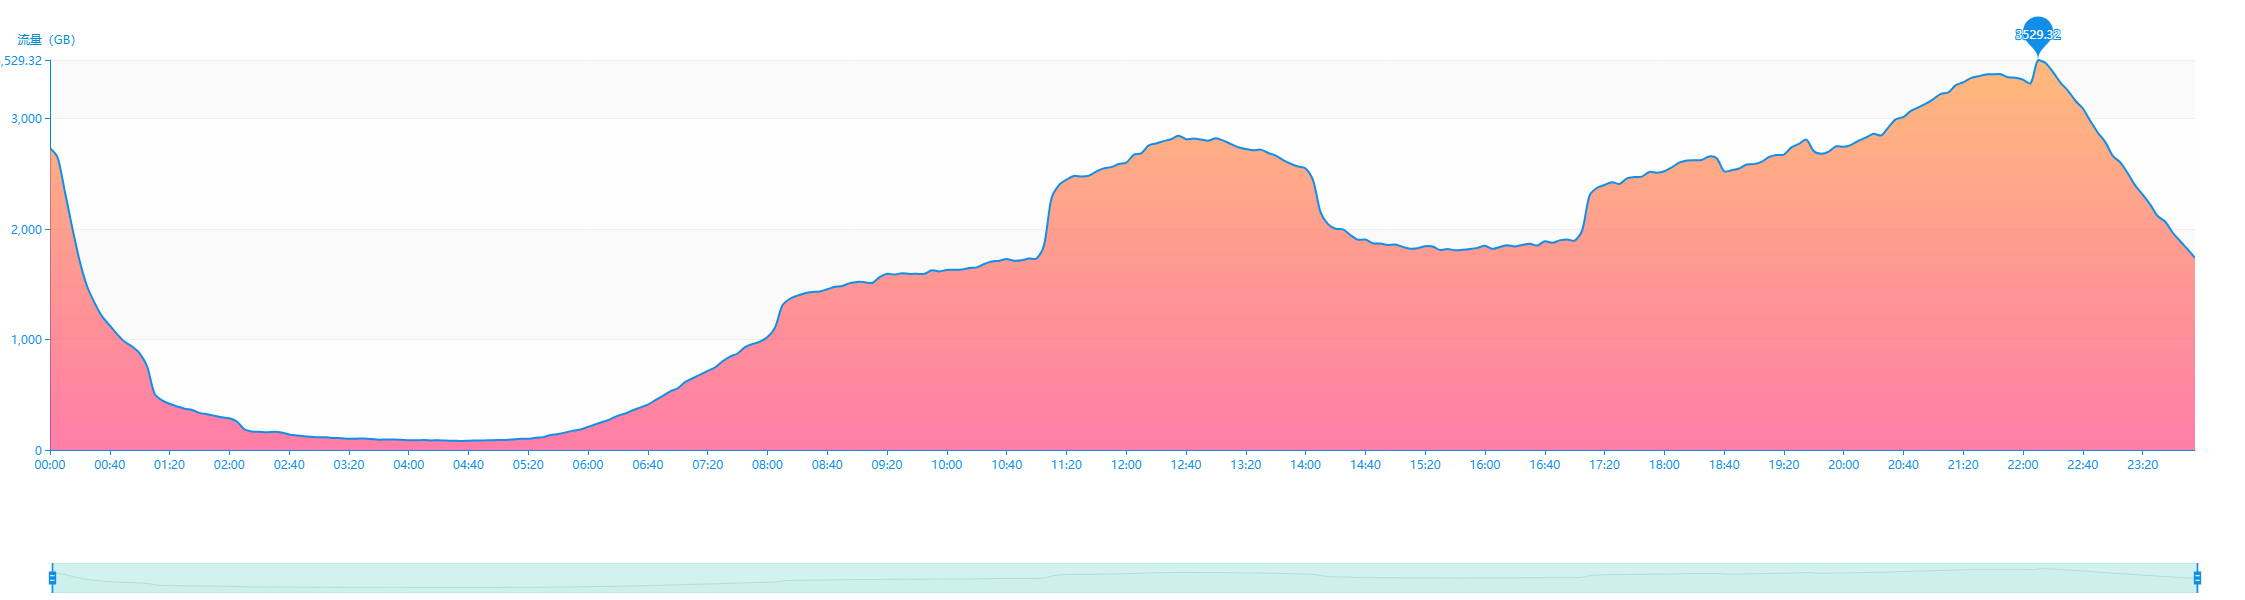
\includegraphics[width= \textwidth]{fig_1.png}
\caption{User traffic in five minutes from tencent video}
 \label{fig_1}
\end{figure}

\section{Fog Computing}
"Fog-based Concent Delivery Network"(Fog CDN), a new video delivery paradigm, which is enabled by fog nodes
(such as Wi-Fi routers,Network Attached Storage,Smart home center,etc.) deployed at users' home, becomes
the most popular topic applying in video replication and access. This  new paradigm is different from
the traditional P2P system, because it's too difficult to operating millions of dedicated
fog nodes  by the centralized video service providers in a coordinative manner\citep{Ma2016Understanding}.
Therefore, a fog-based video delivery and access network would have a huge demand gap.
\subsection{The System Architecture for CDN,P2P And peer CDN}
\begin{figure}[htbp]
\centering
	\vskip 1.0cm
	  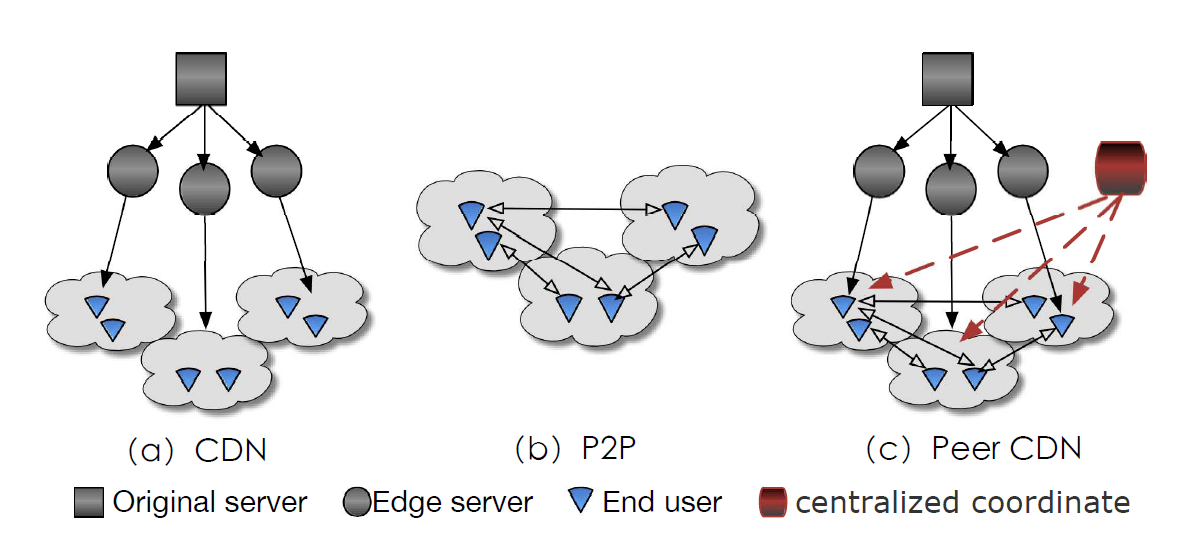
\includegraphics[width= 0.8\textwidth]{fig_2.png}
    \caption{The system architecture for CDN, P2P and peer CDN \citep{Ma2016Understanding}}
	\vskip 1.0cm
 \label{fig_2}
\end{figure}
In Figure \ref{fig_2}, it plot today's content delivery paradigms including conventional CDN,
P2P and peer CDN. Compared with the conventional CDN approach, peer
CDN employs network resources which are much closer to
users, while compared to the conventional P2P paradigm
where users individually cache and serve each other, the nodes
in a peer CDN are closely coordinated by the centralized
knowledge. For example, the content providers schedule nodes
in a peer CDN to proactively cache content, and redirect users
to download content from particular fog nodes. Today, traditional
content providers and such peer CDN providers even
start collaborating to change the traditional content delivery
paradigm, to satisfy the ever increasing generated content and
edge network requests \citep{Ma2016Understanding}.
\subsection{Fog Computing}
Research on fog computing is still in very early stages. On 19 November 2015,
ARM, Cisco, Dell, Intel, Microsoft and Princeton University formed the OpenFog Consortium.
It plans to set up seven different working groups aiming at solving problems in
fog computing, but so far it has only published one architectural white paper \citep{Cheng2014RFC}.

To integrate with the grid and interoperate with other systems, there are problems
like synchronisation and voltage control remaining to be solved. All of them require
replacement of hardware. In contrast, most fog problems lie in the software layer
and can be easily solved by complying with unified protocols. Because of the RTT-throughput
relationship(See Appendix \ref{chap:appA}) and fog’s inherent proximity to the sensors at a local environment,
 the demand for fog computing keeps growing.

\section{Development of Hardware}
In the past few years, we have witnessed the explosive growth of fog devices, as well as
their utilities and functionalities.
\subsection{IoT andWearable: Barrier and Standardisation}
In the past few years, many people have swarmed into the field of wearable devices.
However, we have also witnessed a falling of the tide. For wearables, the bottleneck is
the batteries, which require a significant breakthrough in another domain, which is not
predictable.
On 13 January 2014, Google acquired Nest for USD 3.2 billion. This acquisition triggered
a swarm into the Smart Home concept. Although people have tried IoT for many
years, Apple even emphasising it in late 1970s, the largest barrier to IoT’s market penetration
is the disunity in standard protocol adoption. Each manufacturer has used its
own proprietary protocols and technologies and has been unwilling to be connected to
(let alone controlled by) something from another vendor. The good news \citep{Bille2016RTCSS} is that we are
starting to see some moves towards standardisation.
\subsection{Smart Routers}
On 23 April 2014, XiaoMi launched an OpenWrt-based smartWi-Fi router with 1TB NAS.
It was a landmark event that motivated a lot of hardware vendors as well as Internet
software service companies to crowd into this market. Lenovo introduced NewWiFi, also
on top of OpenWrt. Huawei released Honor Router, which runs a proprietary version
of embedded Linux. Google announced OnHub, which runs Chrome OS. All the three
became “phenomenal products”. They have tried to penetrate the market with smart Wi-
Fi routers due to two main factors:
 \begin{itemize}
 	\item Wireless routers are entry points of users’ data traffic.
  \item Wireless routers are control centres in smart homes.
 \end{itemize}
However, we have now reached a turning point. "MediaTek" (MTK), the fourth largest
fabless IC designer in the world has been powering its Wi-Fi router SoCs with the ARM
Cortex architecture, which is the same as that of the CPUs used in most smartphones,
tablets and TV-boxes.

From a partner company specialising in ODM solutions for routers, we have learned
that MTK has launched a new wireless chipset product-line using the said ARM architecture.

In the Cloud, it is an access point working at the edge; in Home Entertainment, it is a
media centre; in the IoT, it is a controller of all sensors; in the Fog, it is a member of the
distributed service pool.

Briefly speaking, a fog node is a micro data centre that descends the intelligence and
resources from the core to the edge of the Internet, enabling the innovative capabilities to
provide novel and refined applications and services.

\subsection{Larger Memory and Storage at Lower Prices: A Continuous Trend}
According to the Moore's law(Figure \ref{fig_3}), the DRAM costs are dropping about 32\% every 12
months. These would be a support for bringing large buffering, caching, and storage
capacity to edge devices.

\begin{figure}[htbp]
	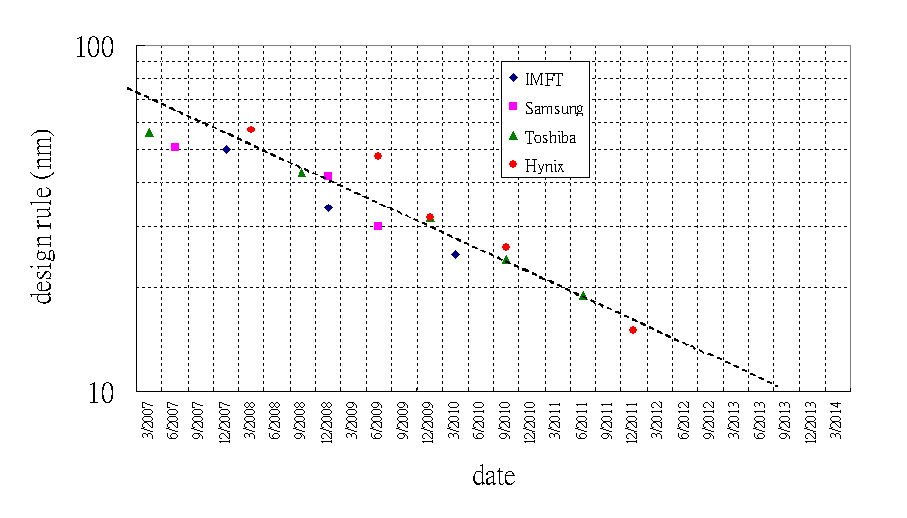
\includegraphics[width=0.8\textwidth]{fig_3}
	\caption{The trend of scaling for NAND flash memory }
	\label{fig_3}
\end{figure}

 \chapter{Related Works}
\label{chap:chap-two}
Some major video content providers and startup companies have used fog-based
video distribution platform. In this chapter, we overview 2 commercially deployed fog-based
video content distribution system: Youku Smart-router  and Thunder Crystal.
Both of them support wired network and deploy the fog resource in users'home,
but they still have some differences.

\section{Smart-router-based Peer Video CDN of Youku}
Youku, one of the largest online video content providers in China \citep{Li2011Measuring}, has deployed over
300K smart-routers in the homes of its end users, expecting that a large fraction of such fog
devices can act as content delivery peer nodes. In this peer CDN system with agents (fog
devices), Peer CDN control servers and CDN Infrastructure, the HTTP protocol is used to
download contents from edge servers, and a private P2P protocol based on UDP, is adopted
for the peers to deliver their data. A smart-router downloads the content from multiple
peers in parallel when it obtains the peer list. We describe the approaches Youku uses to
deal with the major challenges as follows. Youku has not yet published how they operate the
fog network. The understanding of its fog comes from the measurement work to monitor the
traffic of Youku's router \citep{Ma2016Understanding}.

Youku subsidized its users to deploy the smart-routers. Each smart-router has additional
functions (e.g., set-top box, Wi-Fi access points) with lower price. Users with the smart-
routers can also get extra benets (reduction in membership fee) from uploading the contents
with users' bandwidth. We describe the approaches Youku uses to deal with the major
challenges on video replication (Section \ref{subsection_1}) and access (Section \ref{subsection_2})
as follows.

\begin{figure}[htbp]
\centering
	  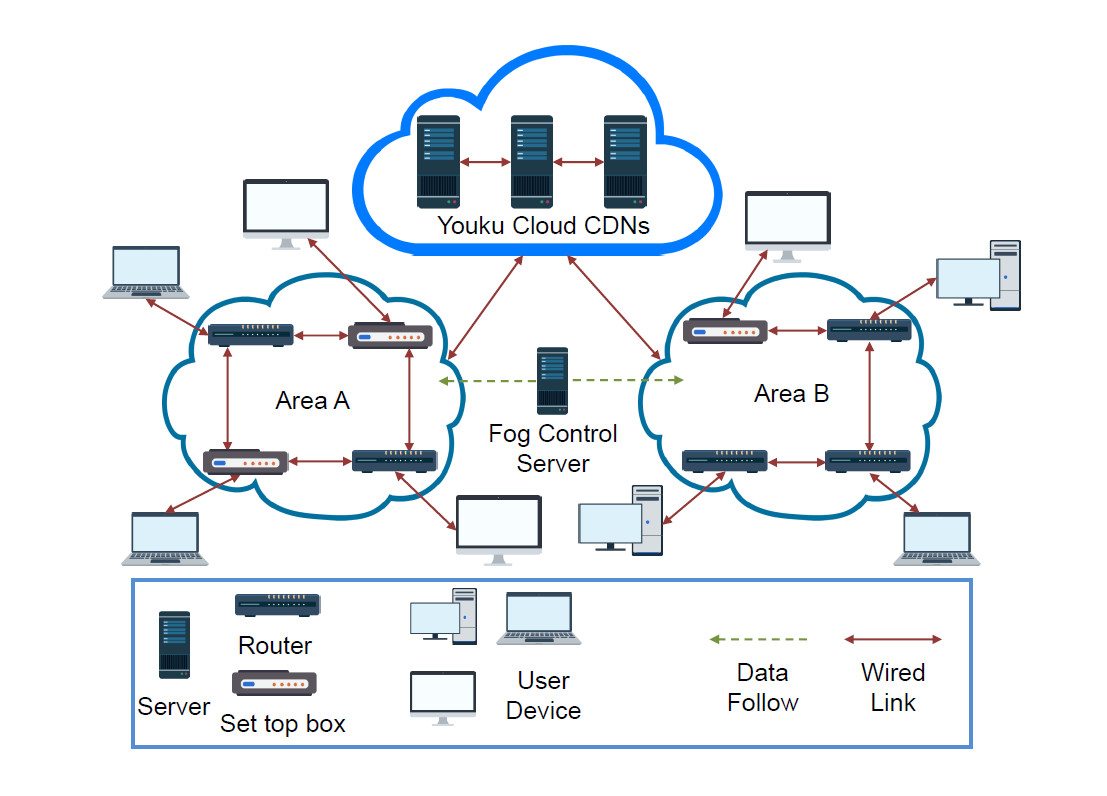
\includegraphics[width=\textwidth]{fig_4.png}
    \caption{Architecture of the peer CDN system of Youku}
 \label{fig_4}
\end{figure}


\subsection{Combing Replication with Recommendation}
\label{subsection_1}
Youku uses a centralized content replication strategy. Both the content push and content
removal are scheduled by the centralized control. Video popularity is the most critical
infuential factor in the video placement. The videos that are popular in the recent month are
likely to be replicated in smart-routers, e.g., over 60\% of the peer-videos are among 1200 most
popular videos of the recent month. Youku content replication strategy is insensitive to the
local content popularity and scheduled globally. However, Youku combines the replication
strategy with its recommendation system.

Video recommendation means the recommendation of videos by Youku, e.g., the homepage
 of Youku generally presents the newly published videos, recommended videos and popular
 video links, which can attract users to click. It is observed that 73\% of the videos
stored by our peer routers are on the homepage, and TV series and cartoon have the highest
possibility to be stored by smart-routers when they are recommended.

The downloaded chunk number follows a daily pattern, i.e., the lower levels of chunk
downloaded happen between 5 and 7 A.M. and 2 and 4 P.M. every day, and the peaks happen
between 0 and 3 A.M., which indicates that chunk downloading is scheduled periodically (i.e.,
hourly) during a day. It is likely that Youku makes replication decision on a daily basis and
push the contents during the time when the Internet traffic level is low.

\subsection{Centralized User Access Coordination}
\label{subsection_2}

The coordinating system in Youku is highly centralized. Youku has 4 kinds of servers to
manage the smart routers:
\begin{itemize}
	\item Config servers: Peer routers download configuration parameters from Config servers.
  \item QoS monitors: Peer routers report statistics to the QoS monitor server, including the
information of their partners and their operation states.
  \item Scheduling servers: Scheduling servers schedule the content replication according to the
information monitored.
  \item Agent managers: A set of agent managers is deployed in different ISPs and locations,
where each of them manages the smart-routers that are close to it.
\end{itemize}

As it seems that Youku do not care about the local content popularity, the control servers
can give similar instruction on all the fog devices. The fog devices usually store the similar
popular contents, so the users only need tond the nearest available fog device for the video
contents. The agent managers can make sure that users mostly request the content with the
same ISP domain.

\section{Thunder Crystal: Crowd-sourcing Content Distribution}

Thunder (Xunlei) is a popular P2P file sharing client side software in China \citep{Dhungel2011Measurement} \citep{Dhungel2012Xunlei}. To
extend their business, their users who have installed Thunder software (which are called
agents) can help some video content providers to distribute the content for monetary return.
The operator of Thunder Crystal, together with some researchers, has published some work
to illustrate how Thunder Crystal works \citep{Chen2015Thunder}.

In this work \citep{Chen2015Thunder} the Thunder Crystal is called a crowdsourcing system. In Thunder Crystal,
 Thunder asks some users (agents) with surplus bandwidth and computing resources to
support its content delivery. Unlike traditional P2P paradigm, Thunder's cloud servers have
the right to keep pushing content to agents if the agents agree to contribute their storage (to
store content) and upload bandwidth (to distribute content to end users) by rebated cash
from Thunder Crystal. Each agent is like a mini-CDN edge server, which is very close to end
users.

Most agents are normal Internet users who would like to offer their surplus bandwidth
with very low charge, but a user can have a better price by contributing their bandwidth in
peak hour. However, with the current price, it is enough for a user to cover its electricity
and network utility bills. Compared to the charging policies of the CDN companies, the
cash rebated to agents is much lower, implying lower expenses for distribution service. We
describe the approaches Thunder uses to deal with the major challenges on video replication
(Section \ref{subsection_3}) and access (Section \ref{subsection_4}) as follows.
\begin{figure}[htbp]
\centering
	  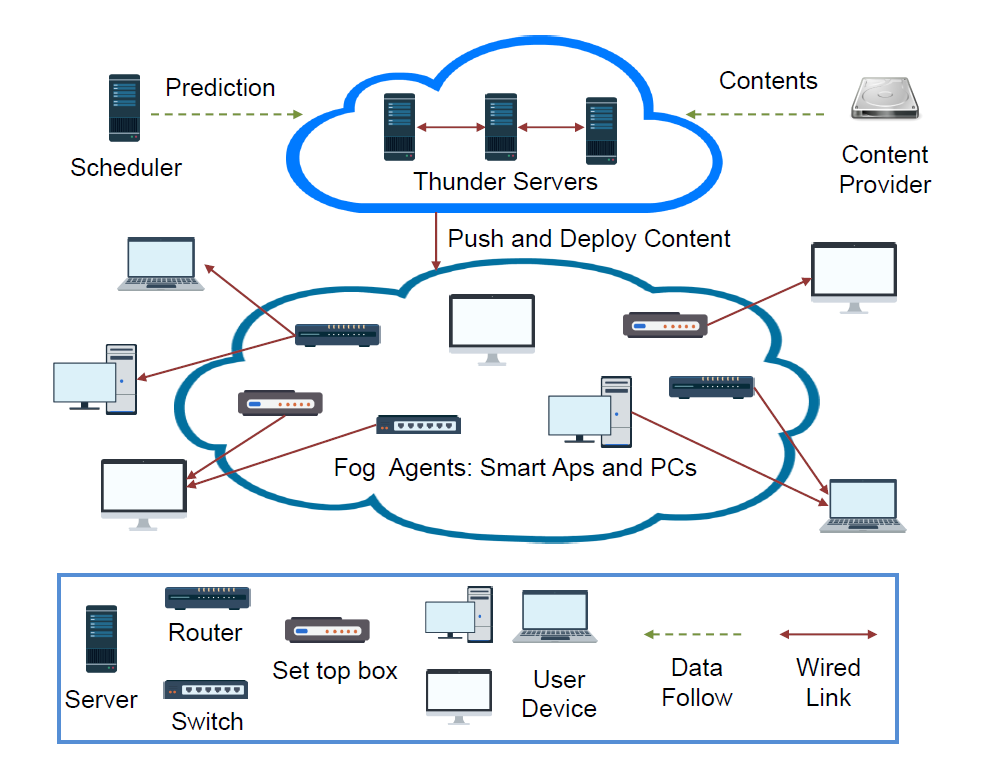
\includegraphics[width=\textwidth]{fig_5.png}
    \caption{System overview and general architecture of Thunder Crystal}
 \label{fig_5}
\end{figure}


\subsection{Replication Based on Popularity}
\label{subsection_3}
In Thunder's pushing strategy, agent devices are not discriminated. Thunder servers push
the new replicas randomly to different agent devices. Therefore, the fog network has no
locality awareness. Thunder servers can push 80TB traffic per day as their traffic budget.
Files will be pushed out by decreasing order of popularity until the traffic quota is used up.
In other words, more popularles will be pushed with higher priority than less popular files.
If the storage of an agent is full, thele with the lowest global popularity will be replaced.

To calculate the global popularity, besides the new contents, if the number of requests to
download a file is N, Thunder Crystal will maintain $ (0.05N)^{0.96}$ replications in the next day.
Such formula is obtained from experimental trials.

\subsection{Random User Access}
\label{subsection_4}
In current Thunder Crystal system, there are more than 11K active agent devices, which
is smaller than the scale of Youku. For each agent device, it serves all received requests
with best efforts. For each user, the file downloading is conducted chunk by chunk with
each chunk size 2MB. The first chunk is from the cloud CDN, and the rest of the chunks
will be chosen from around 200 agent devices with the desired content randomly. Therefore,
Thunder Crystal uses random video access scheme, which is not ISP friendly.

A data report module is embedded into the software that installed on the agent devices.
Reported information includes the number of agent devices that are working at any moment,
measured instant uploading speed, event-driven messages recording the access log of content
and other activities. To protect the copyright and avoid the user to falsely report its
contribution, all the files on any agent's fog device are encrypted.

 \chapter{Architecture of Fog VDN}
\label{chap:chap-three}
\begin{figure}[htbp]
\centering
	  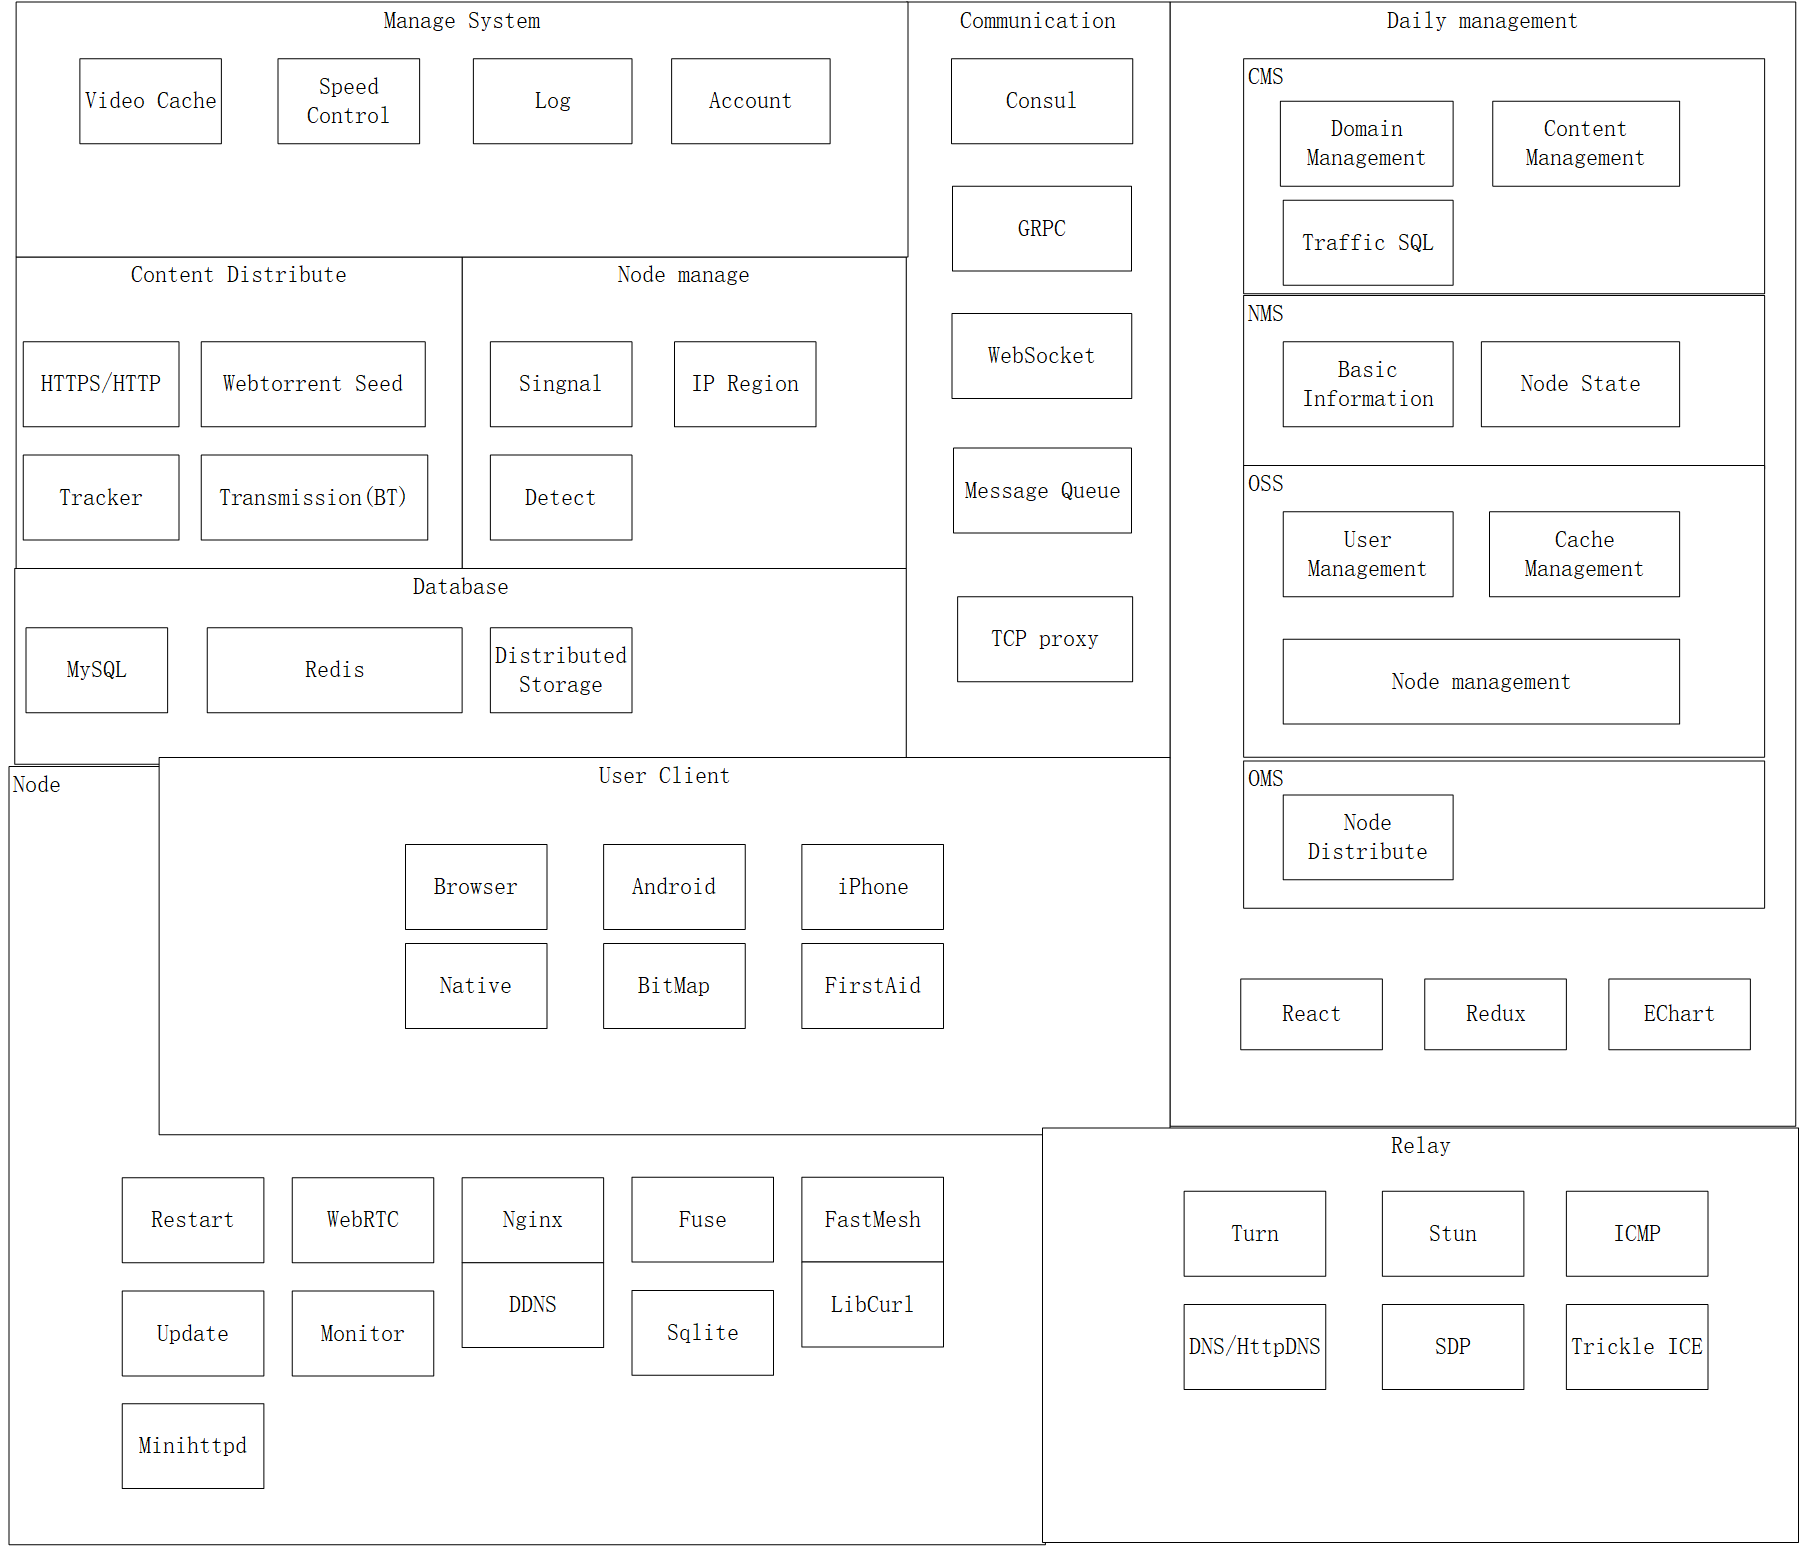
\includegraphics[width=\textwidth]{fig_6.png}
    \caption{Architecture of the Fog VDN}
	  \vskip 1.0cm
 \label{fig_6}
\end{figure}



Fog VDN is very simple(Figure \ref{fig_26}). The fog composed of the fog device
(such as Wi-Fi routers,Network Attached Storage,Smart home center,etc.) collect the
resources (bandwidth,storage,computing) combining cloud server to serve application X
(Fog as a Service FaaS,Figure \ref{fig_27}). But Fog VDN is also complex (Figure \ref{fig_6}),
composed by many systems. Whether simple or complex, Fog VDN has three subsystems,
Node System, Operations Management System and Network Protocols.

\begin{figure}[htbp]
\centering
	  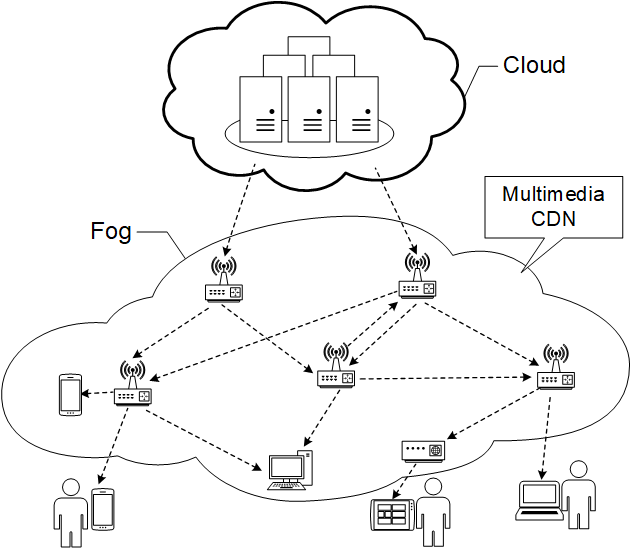
\includegraphics[width=0.8\textwidth]{fig_26.png}
    \caption{Simple architecture of the Fog VDN}
 \label{fig_26}
\end{figure}

\section{Node System}
 \label{Node System}
\begin{figure}[htbp]
\centering
	  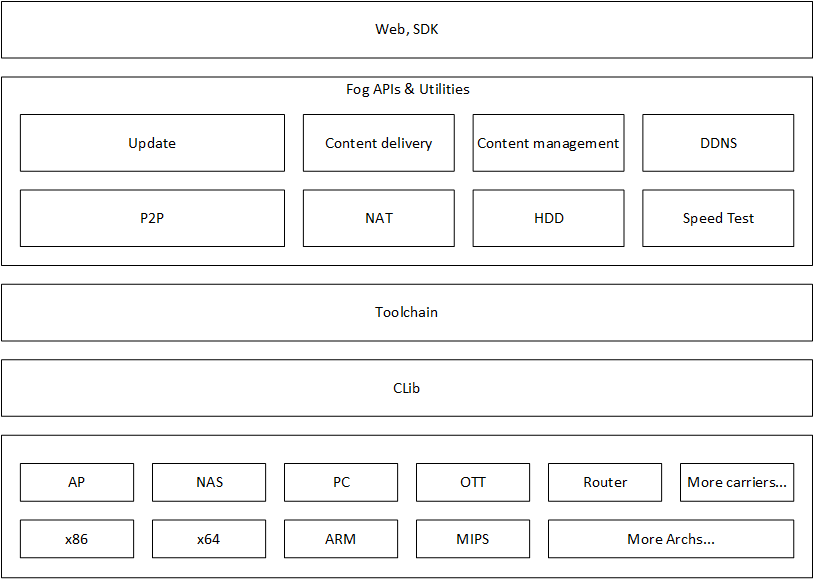
\includegraphics[width=\textwidth]{fig_25.png}
    \caption{ Architecture of the Fog nodes}
 \label{fig_25}
\end{figure}

  \subsection{Fog devices}
    \label{Fog devices}
  There are many different types about fog nodes, "Personal Computer"(PC), "Network Attached Storage"(NAS),
WirelessAccessPoint,Router,Mobile,Base Station all included. In this thesis, we only talk about the fog nodes
which can run the Fog VDN well, which generally have a large storage(>16GB), ROM(>32MB) and RAM(>512MB).
  For hardware devices, there are too many different platforms and configurations to easily unified.
Different from Xunlei and Youku product same hardware, also not same as Huawei use a heavy JVM platform,
 We use the C programing in order to minimize the size of program, so that it can run well in the fog
nodes and we can code once, compile everywhere.
 \subsection{Basic module}
    \label{Basic module}
  \begin{itemize}
    \item Node\_update  : update the program in node.
    \item Node\_restart : restart if the process broken down.
    \item Node\_monitor : monitor the process.
    \item Node\_report  : report the node basic information every 5 minutes.
    \item Node\_p2p     : connect to the other fog node.
    \item Node\_log     : record the node run time information.
    \item Node\_file    : manage the data in the nodes.
  \end{itemize}

  Fig \ref{fig_36} shows the relationship between these basic module.
 \subsection{General fog node}
 One of the most famous design philosophy of peer-to-peer system is sharing. As an application of P2P,
we also inherit the spirit of sharing. A special fog node  means the nodes which we refer to in section
\ref{Fog devices} . A general fog node include not only special fog node, but also the client. Figure
\ref{fig_34} is a fog player client, the red block is downloaded from the cloud, the blue, yellow and green
block is downloaded from special fog node. The purple block is downloaded from the client who is watching
this video. This is general fog node, same as conventional P2P node.
 Fig \ref{fig_25} shows the general fog node architecture.

\begin{figure}[htbp]
\centering
	  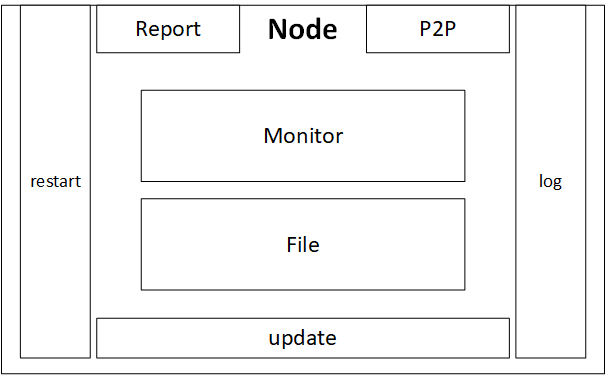
\includegraphics[width=0.8\textwidth]{fig_36.png}
    \caption{ Architecture of the Fog nodes System.}
 \label{fig_36}
\end{figure}

\section{Console}
\subsection{Operations Management System}
 \label{Operations Management System}
 Node system \ref{Basic module} have a basic module called Node\_report. The "Operations Management System"
(OMS) shows the statistics of these information (Figure \ref{fig_29}).
\begin{itemize}
	\item Amount                 : The number of fog nodes (\ref{Fog devices}).
	\item Amount\_online         : The number of fog nodes online.
  \item Bandwidth\_total       : The total upload/download bandwidth of fog nodes.
  \item Bandwidth\_total\_wan  : The total upload/download ability   of fog nodes.
  \item Bandwidth\_avg         : The average upload/download bandwidth of fog nodes.
  \item Bandwidth\_avg\_wan    : The average upload/download ability   of fog nodes.
  \item Storage\_total         : The total storage of fog nodes.
  \item Storage\_total\_able   : The available storage of fog nodes.
  \item NAT\_type              : The "Network Address Translation"(NAT) type.
  \item Platform               : The fog node's platform.
  \item HTTP                   : The node can support http connect.
  \item Version                : The node system version.
  \item Province               : The node province distribution.
  \item ISP                    : The node "Internet Service Provider"(ISP).
  \item Traffic                : The node traffic every 5 minutes.
\end{itemize}
  Figure \ref{fig_37} shows the relationship of these information.

\begin{figure}[htbp]
\centering
	  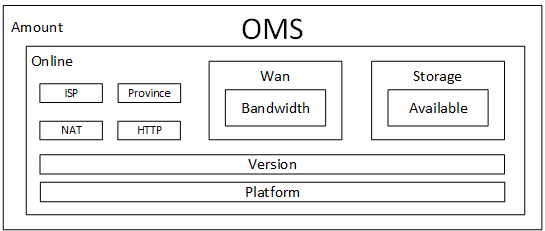
\includegraphics[width=0.8\textwidth]{fig_37.png}
    \caption{ Architecture of the OMS.}
 \label{fig_37}
\end{figure}

\subsection{Operation Supporting System}
The "Operation Supporting System" (OSS) is designed for administrator operating the fog nodes
(Figure \ref{fig_30}, Figure \ref{fig_32}).
\begin{itemize}
	\item Node\_list         :Similar to OSS (\ref{Operations Management System}), specific to each node.
  \item Update             : Update program by province, city, ISP, platform and current version.
  \item Update\_state      : Node update state.
  \item Version            : Node version distribution.
  \item Traffic            : Used traffic.
  \item Bandwidth          :Realtime bandwidth.
  \item Cache\_info        : Show the video uploaded information, include file\_name, host\_name, request\_url, distribute\_scheme, distribute\_status, upload\_time, finish\_time.
  \item Cache\_management  : Include upload, delete, change\_popularity, set\_url.
\end{itemize}


\subsection{Node Management System}
The "Node Management System" (NMS) is designed for user managing their fog device(Figure \ref{fig_38}).
\begin{itemize}
	\item User\_info     : User information include user name, email and phone.
  \item User\_coin     : User rewards for share their fog device.
  \item Node\_list     : User fog nodes list include "Media Access Control"(MAC), "Serial Number"(SN), NAT\_type, platform, version, province, ISP.
  \item Node\_state    : Node online or not.
  \item Node\_config   : Node configure.
\end{itemize}

\section{Application}
 In order to give an example that how to use the fog resource, we opensource a fog player.
Fig \ref{fig_7} show the architecture of this fog player.
\begin{figure}[htbp]
\centering
	  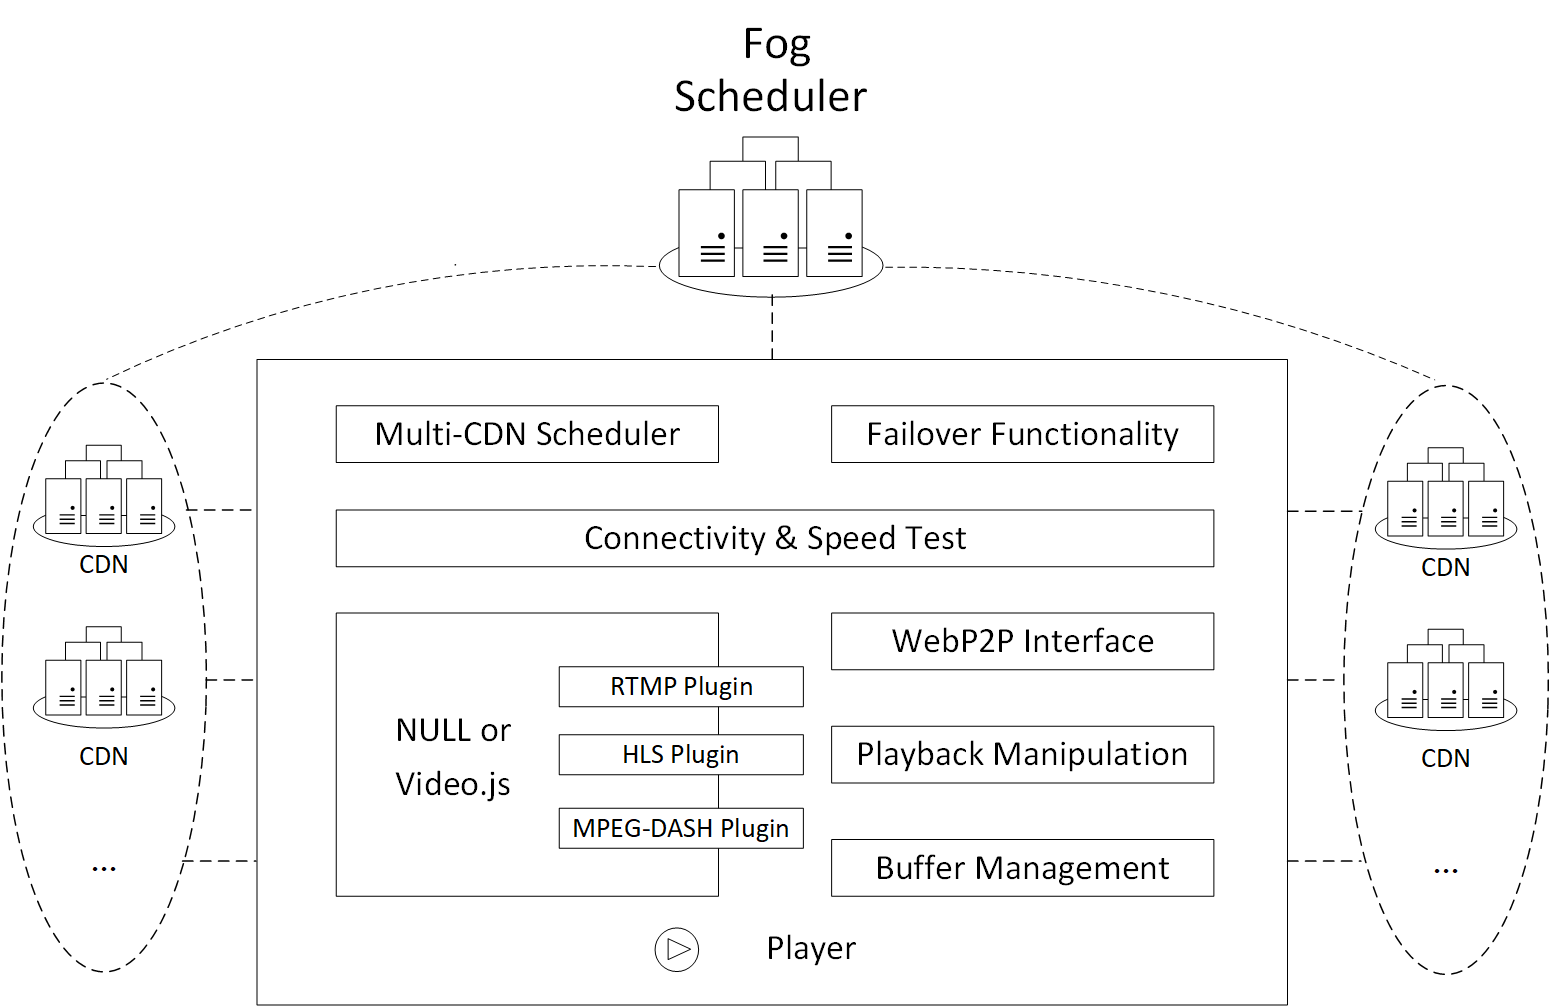
\includegraphics[width=\textwidth]{fig_7.png}
    \caption{Architecture of the Fog Player}
	  \vskip 1.0cm
 \label{fig_7}
\end{figure}

\section{Protocols}
In section \ref{Node System} we show a figure \ref{fig_25} of the architecture of fog nodes.
But if you were careful enough, you would find it is more protocol than system. We try to not only
conding a fog video distribution system but also summarizing a "Fog Video Distribution Network"(Fog VDN)
which focuse on protocol.Figure \ref{fig_8} and Figure \ref{fig_17} shows the fog node engine and Fog VDN stack.

Though we realized a fog video distribution sysem, and try to summarize some standards of connecting
the fog nodes as a network. But it is far away from a protocol, we still have a long way to go.


\begin{figure}[htbp]
\centering
	  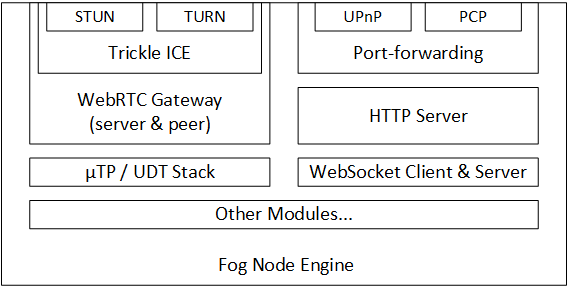
\includegraphics[width=0.8\textwidth]{fig_8.png}
    \caption{Architecture of the Fog Node Engine}
 \label{fig_8}
\end{figure}

\begin{figure}[htbp]
\centering
	  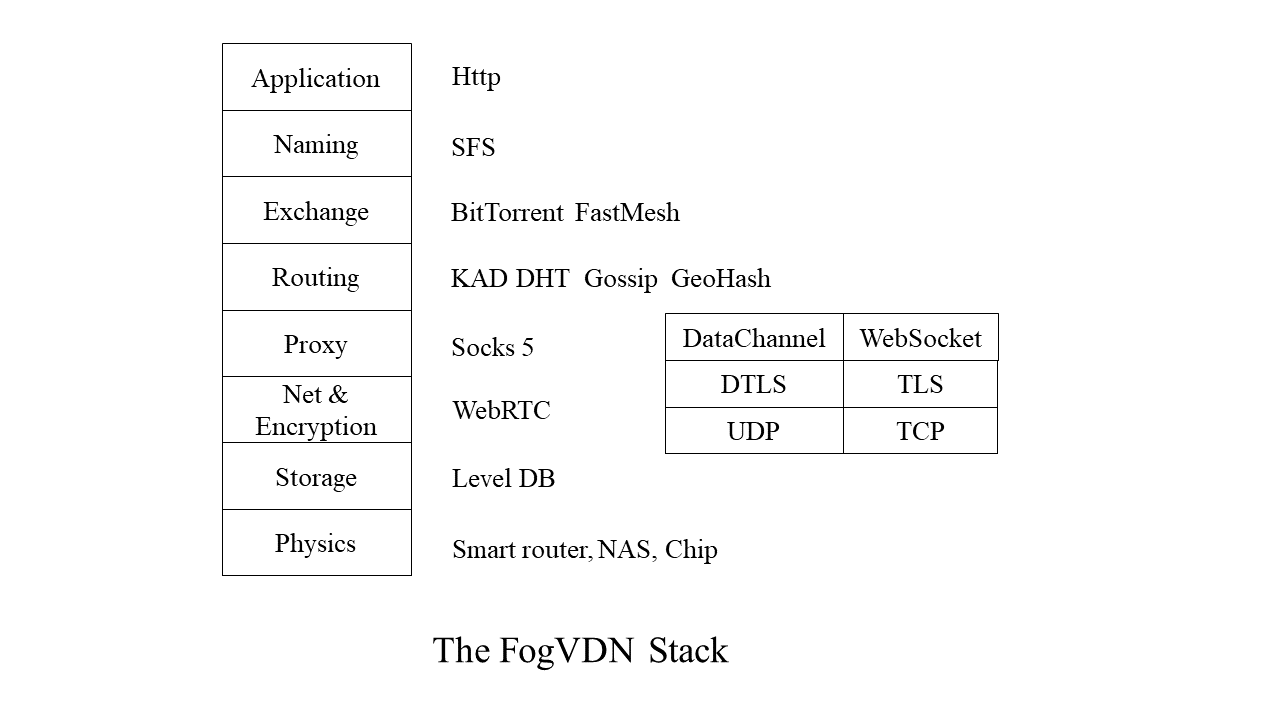
\includegraphics[width=\textwidth]{fig_17.png}
    \caption{Fog VDN Stack}
 \label{fig_17}
\end{figure}

 \chapter{Results}
\label{chap:chap-four}
\section{Node ability test}
\subsection{Nodes upload test}
 Test 40,000 nodes'(random select) speed  three times a day (3A.M. Figure \ref{fig_20} ,
12A.M. Figure \ref{fig_21} , 9 P.M. Figure \ref{fig_22})
by uploading a big file (1GB) to the server, using TCP connect.


\begin{figure}[htbp]
\centering
	  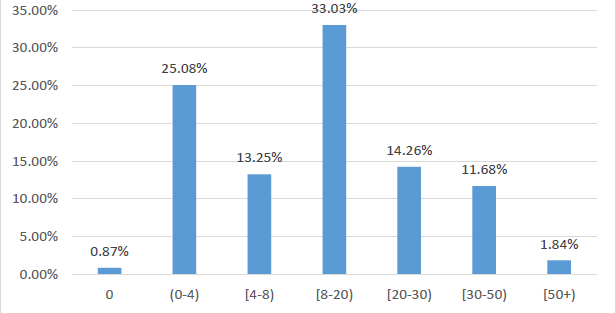
\includegraphics[width=\textwidth]{fig_20.png}
    \caption{3 A.M.}
 \label{fig_20}
\end{figure}

\begin{figure}[htbp]
\centering
	  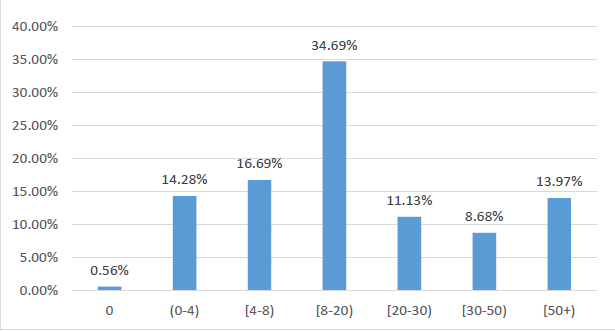
\includegraphics[width=\textwidth]{fig_21.png}
    \caption{12 A.M.}
 \label{fig_21}
\end{figure}

\begin{figure}[htbp]
\centering
	  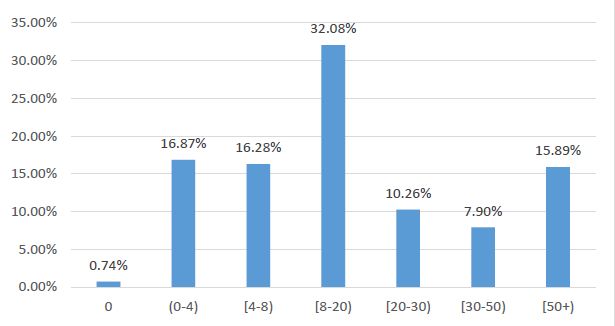
\includegraphics[width=\textwidth]{fig_22.png}
    \caption{9 P.M.}
 \label{fig_22}
\end{figure}

\subsection{One node serve ability base test}
In "Local Area Network"(LAN), different request size, different parallel request amount,
record the upload speed (KB/S)(Figure \ref{fig_28}).

\begin{figure}[htbp]
\centering
	  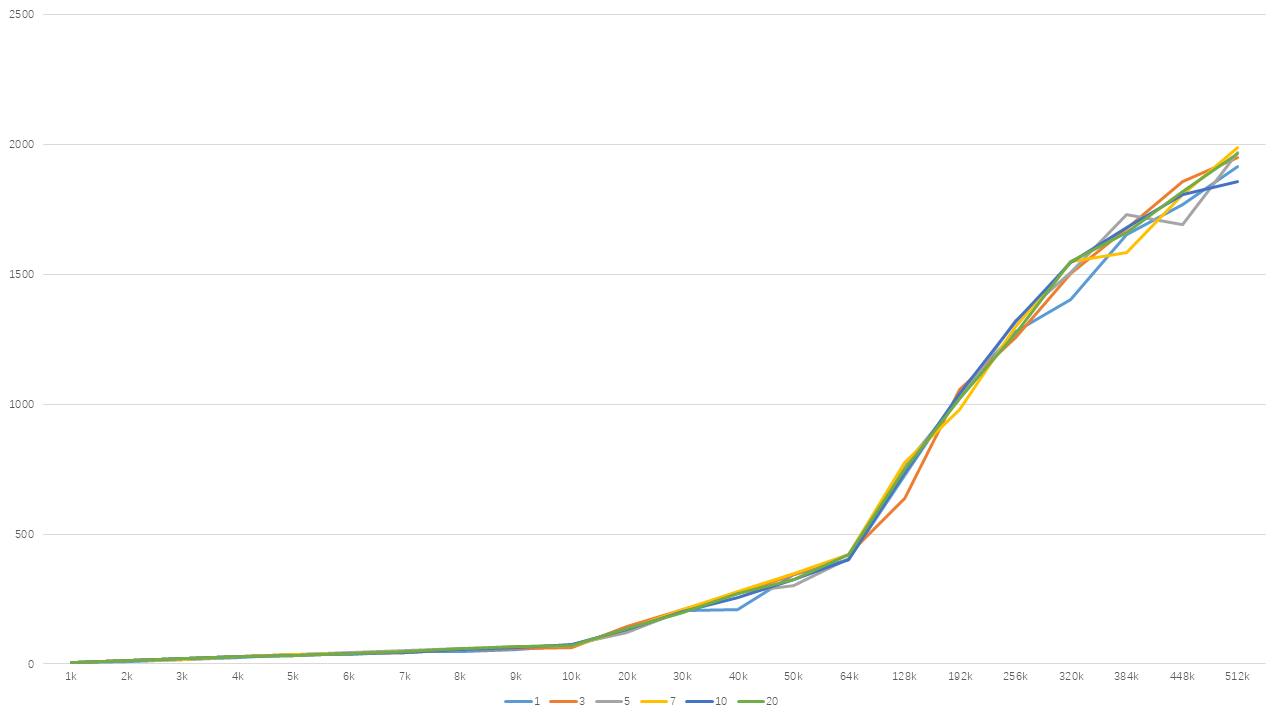
\includegraphics[width=\textwidth]{fig_28.png}
    \caption{One node serve ability base test}
 \label{fig_28}
\end{figure}

\section{File deliver test}

Random select 912 nodes, deliver file size 203M, count the downloaded nodes every 10 minutes
(Figure \ref{fig_23}).
\begin{figure}[htbp]
\centering
	  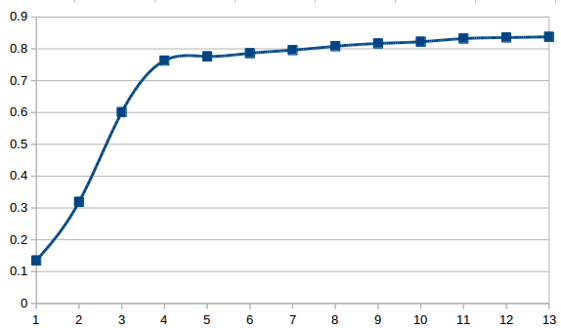
\includegraphics[width=\textwidth]{fig_23.png}
    \caption{File deliver test}
 \label{fig_23}
\end{figure}

 \chapter{Conclusions and Discussion}
\label{chap:conclusion}

  %自行添加

%
%
%  \include{chapter/chap-five}
%  \include{chapter/chap-six}
%  \include{chapter/chap-seven}
%  \include{chapter/chap-eight}
%


%%%%%%%%%%%%%%%%%%%%%%%%%%%%%%
%% 附件部分
%%%%%%%%%%%%%%%%%%%%%%%%%%%%%%
\backmatter
  %结语

  % 参考文献
  % 使用 BibTeX
  % 选择参考文献的排版格式。注意ustcbib这个格式不保证完全符合要求,请自行决定是否使用
  \bibliographystyle{sustcbib}%{GBT7714-2005NLang-UTF8}
  \bibliography{bib/tex}
  \nocite{*} % for every item
  % 不使用 BibTeX
  % \include{chapter/bib}



  % 附录,没有请注释掉
  \begin{appendix}
%  \chapter{User Incentive}
\label{chap:appD}
\begin{figure}[htbp]
\centering
	  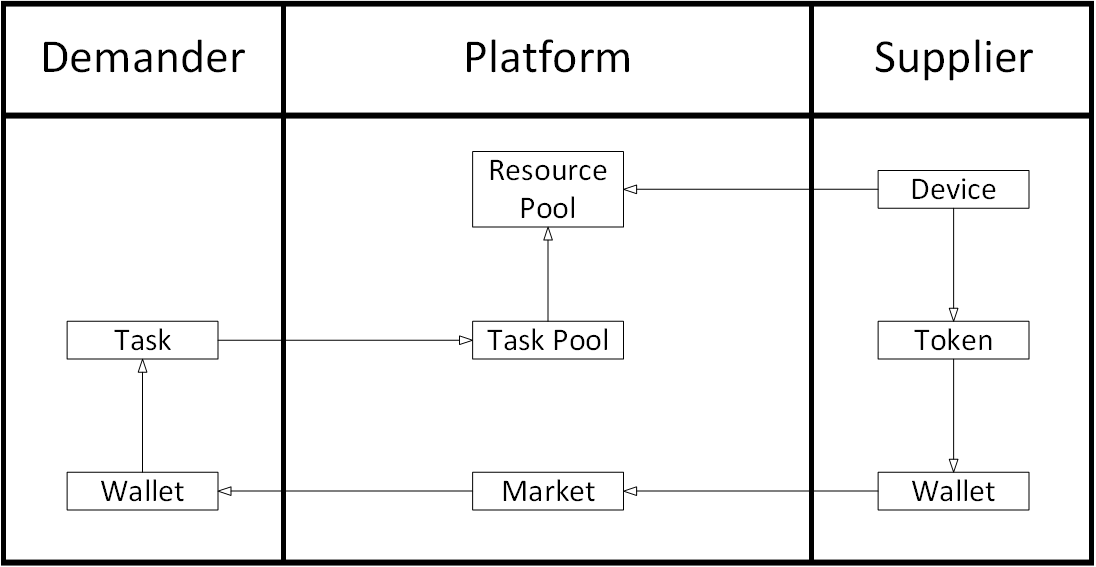
\includegraphics[width=\textwidth]{fig_16.png}
    \caption{Ecosystem Model}
 \label{fig_16}
\end{figure}


  \chapter{The TCP Throughput}
\label{chap:appA}
It is known to all networking professionals that Equation \ref{equ_tcpthroughput}
below is the throughput TCP can achieve at a steady state,
Equation \ref{equ_tcpthroughputmax} is roughly the maximum throughput TCP
can achieve.
\begin{equation}
 \label{equ_tcpthroughput}
  Throughput_{TCP}=\frac{min(RWND,CWND)}{RTT}
\end{equation}
\begin{equation}
 \label{equ_tcpthroughputmax}
  Throughput_{TCP_{max}}=\frac{RWND_{max}}{RTT}
\end{equation}
where RWND is the receiver window size, CWND is the congestion windows size (at the
sender side), and RTT is the round trip time.
Also, theoretically we have Equation 2.3 if considering the loss rate p.
\begin{equation}
 \label{equ_tcpthroughputmax}
  Throughput_{TCP} \approx \frac{1}{RTT}\sqrt{\frac{3}{2p}}
\end{equation}
Let’s consider transmitting a data chunk from node A to node B. When the distance
between A and B gets longer, generally the RTT is larger for a certain type of transmission
medium. In addition, p is also likely to be larger, as there are likely to be more routers
along the path from A to B, and their performance, buffer window sizes, and current
congestion status may vary. Thus, any single node in between can be a bottleneck.
In addition to the window sizes, the packet loss rate p, and the RTT, there are other
factors that affect TCP’s performance: the slow-start and the 3-way handshake behaviour.

  \chapter{More Architectures}
\label{chap:appB}
\begin{figure}[htbp]
\centering
	  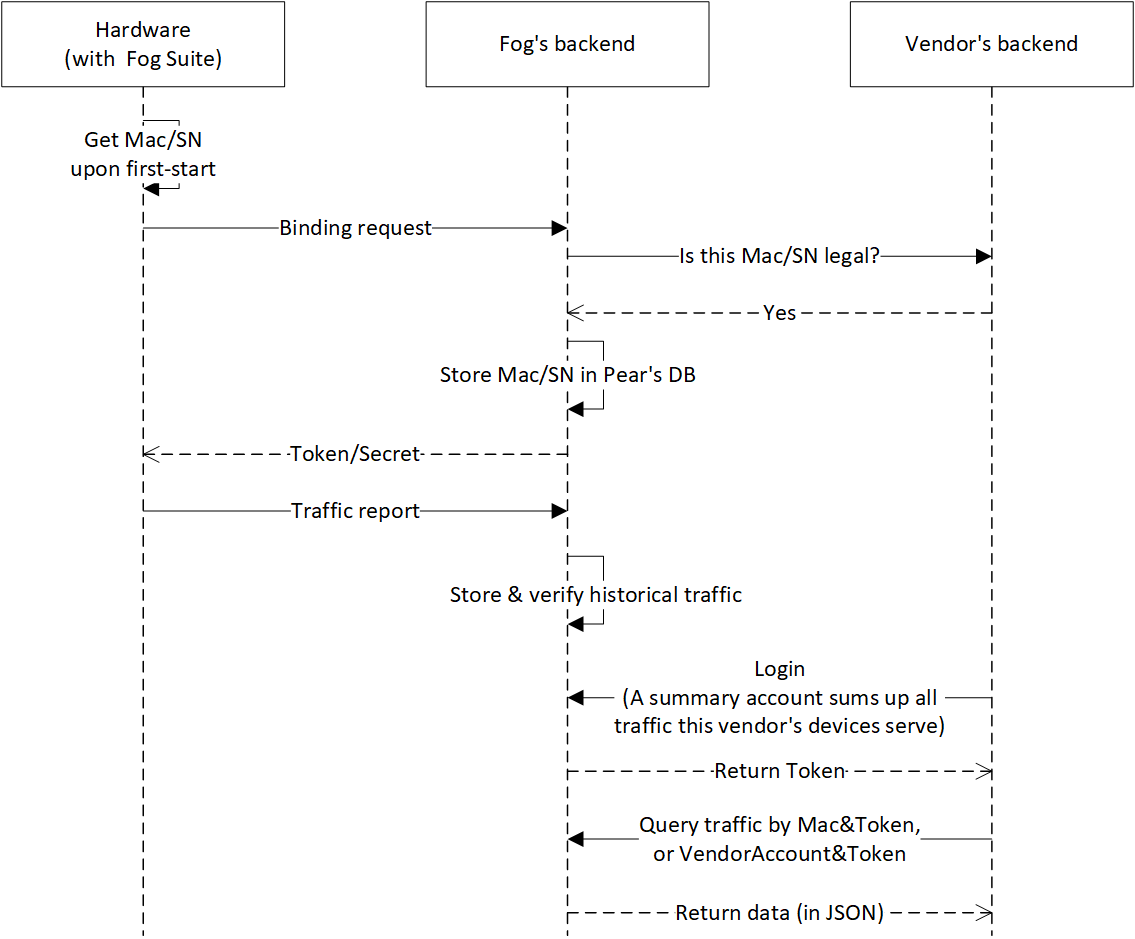
\includegraphics[width=\textwidth]{fig_9.png}
    \caption{Architecture of the Fog Node Bind}
 \label{fig_9}
\end{figure}

\begin{figure}[htbp]
\centering
	  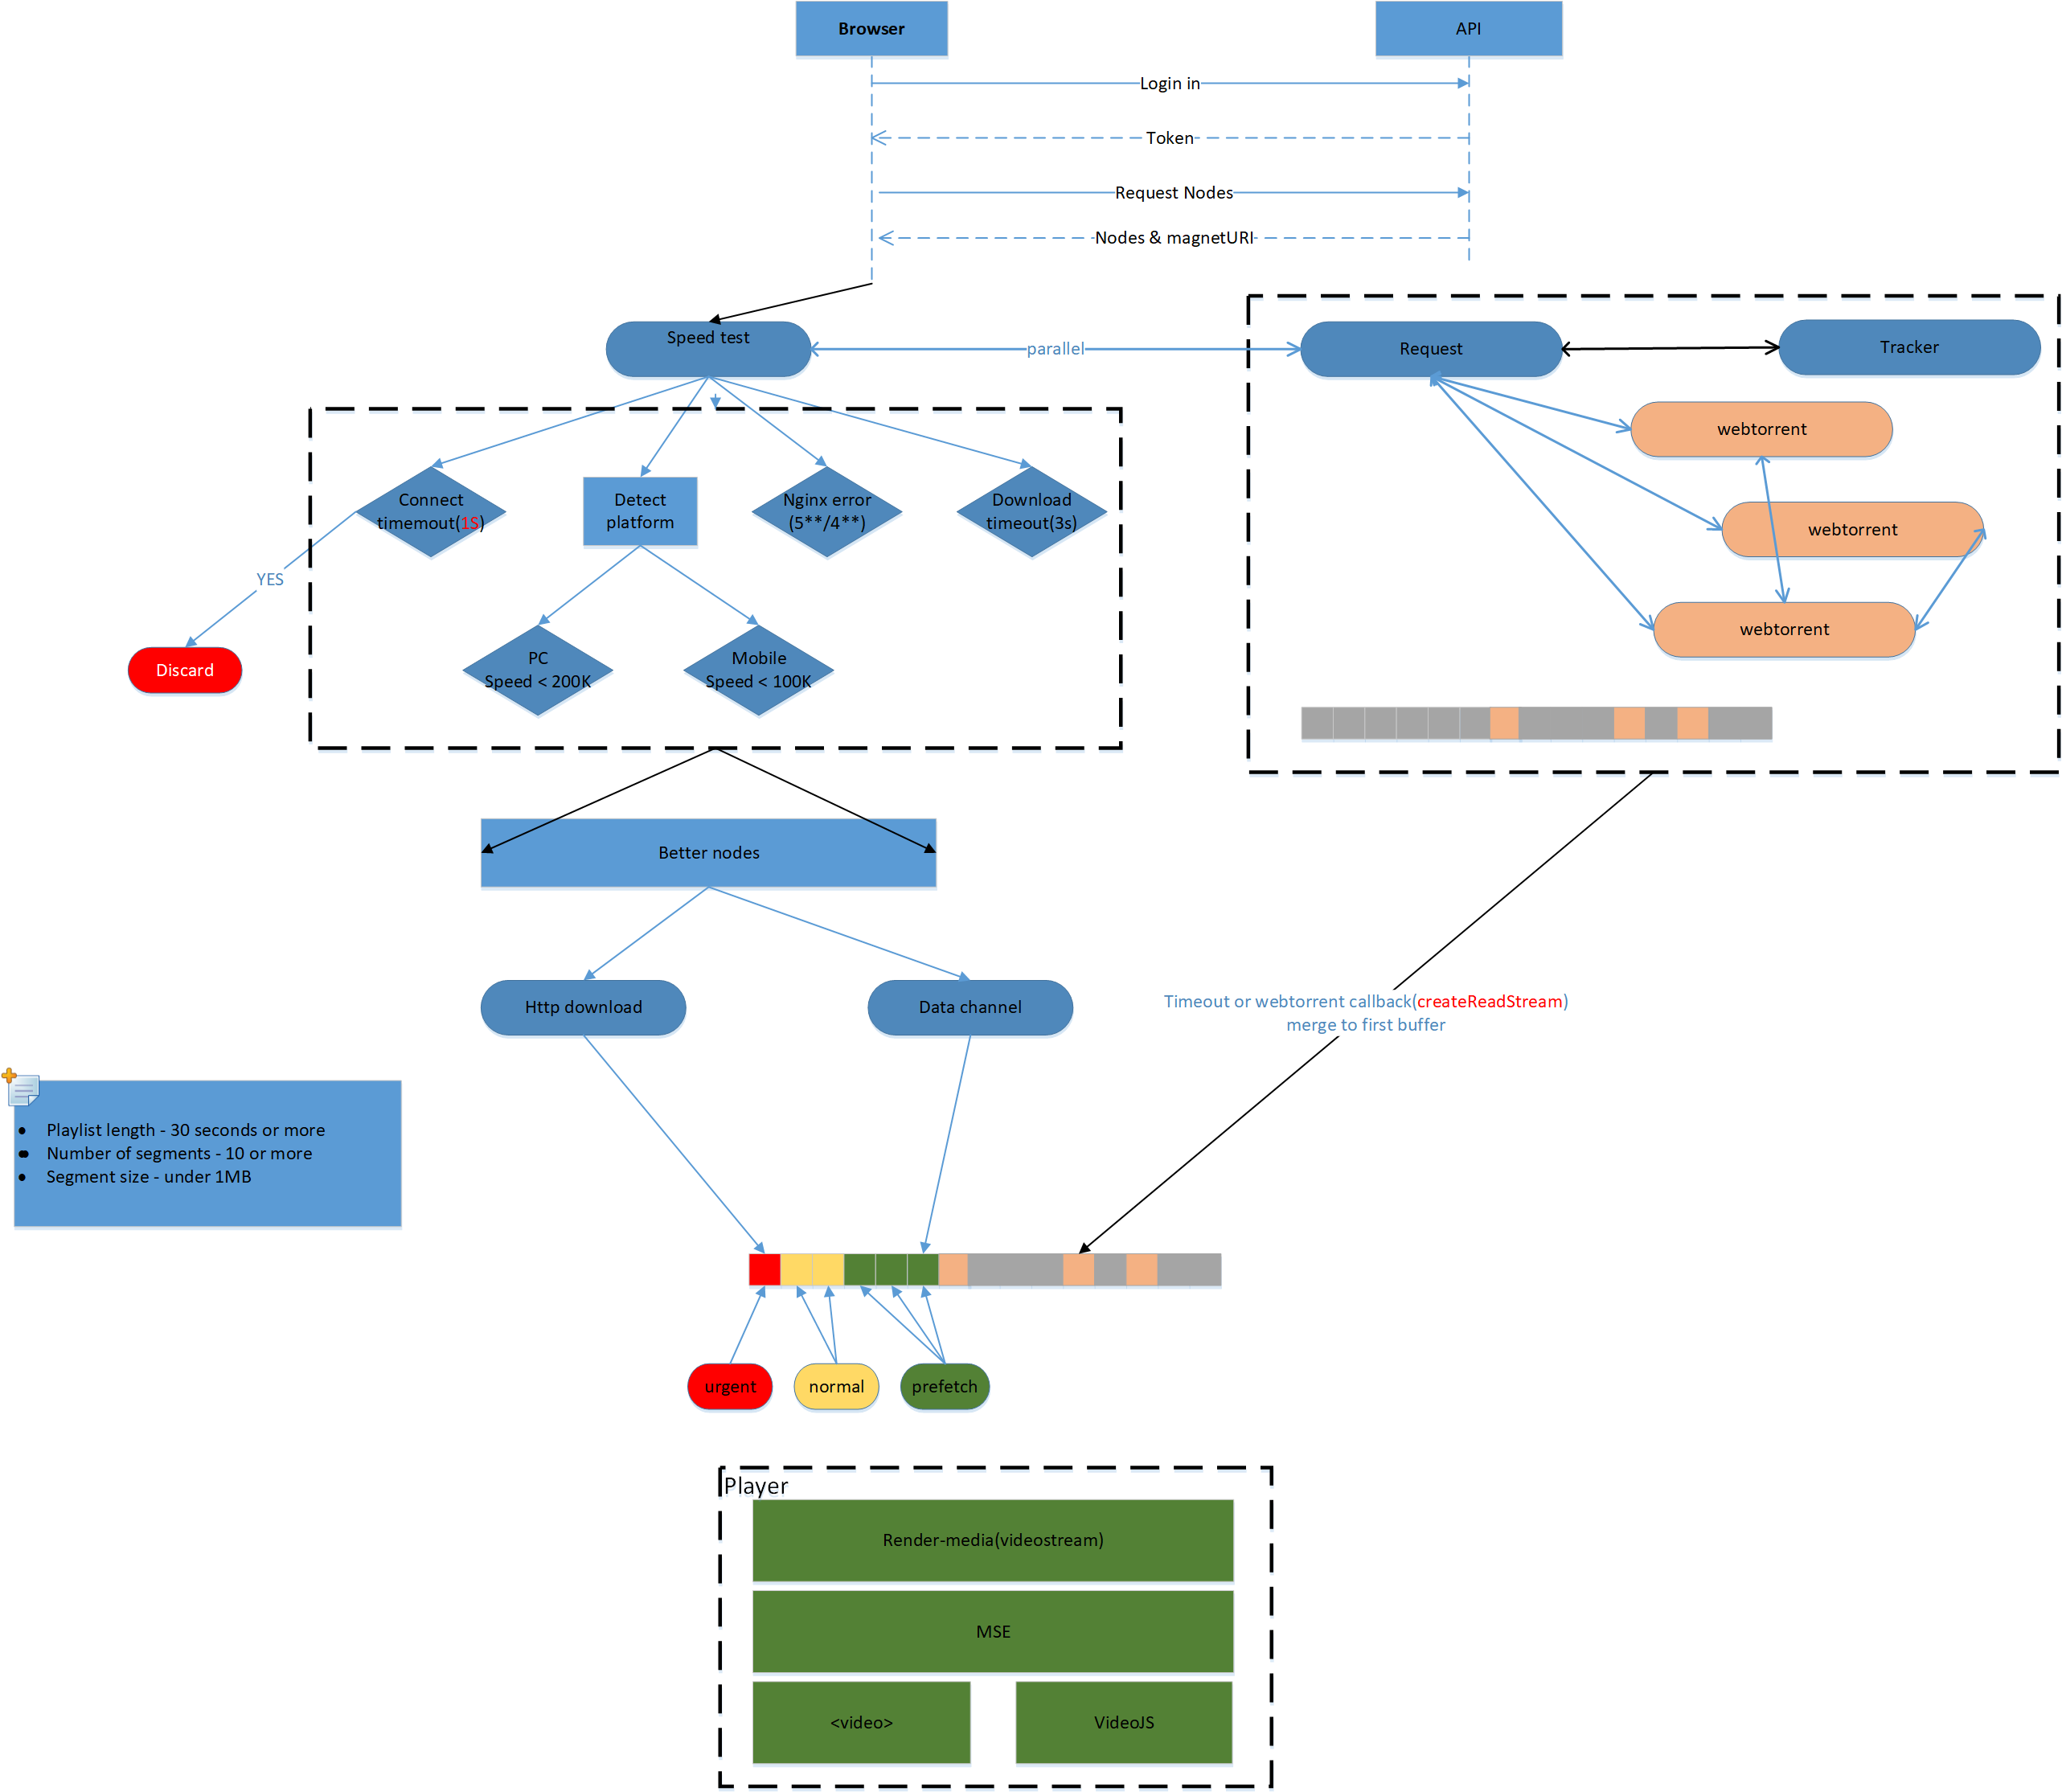
\includegraphics[width=\textwidth]{fig_10.png}
    \caption{Architecture of the Fog Player-1}
 \label{fig_10}
\end{figure}

\begin{figure}[htbp]
\centering
	  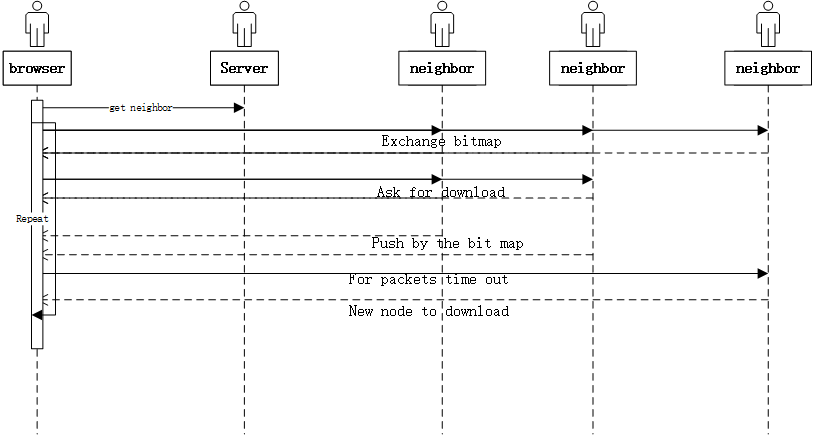
\includegraphics[width=\textwidth]{fig_14.png}
    \caption{Architecture of the Fog Player-2}
 \label{fig_14}
\end{figure}

\begin{figure}[htbp]
\centering
	  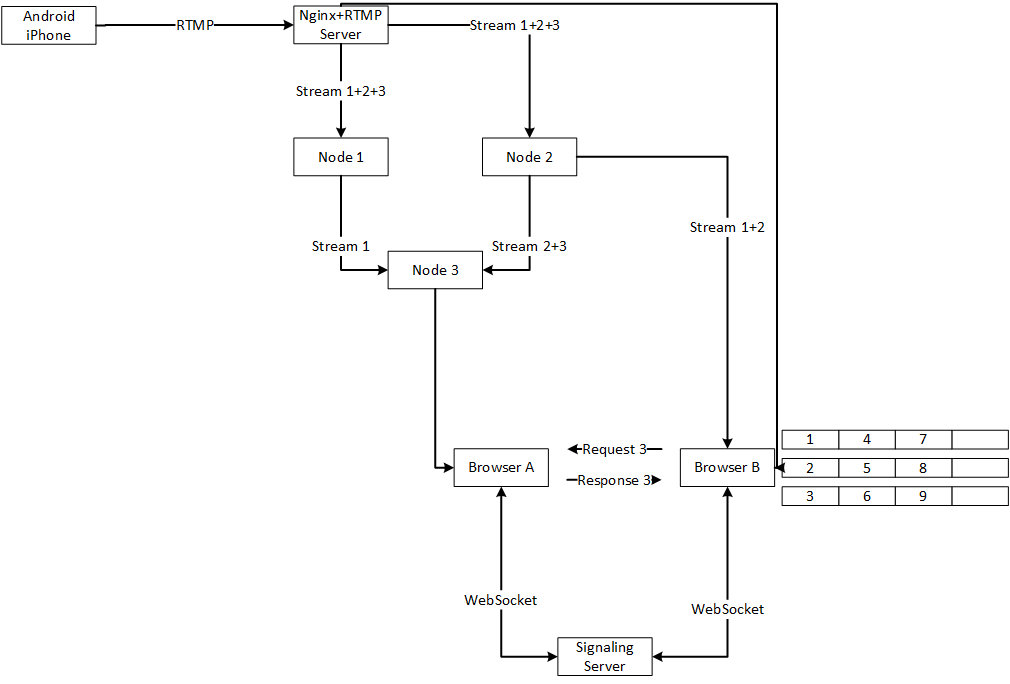
\includegraphics[width=\textwidth]{fig_13.png}
    \caption{Architecture of the Fog Player-3}
 \label{fig_13}
\end{figure}
\begin{figure}[htbp]
\centering
	  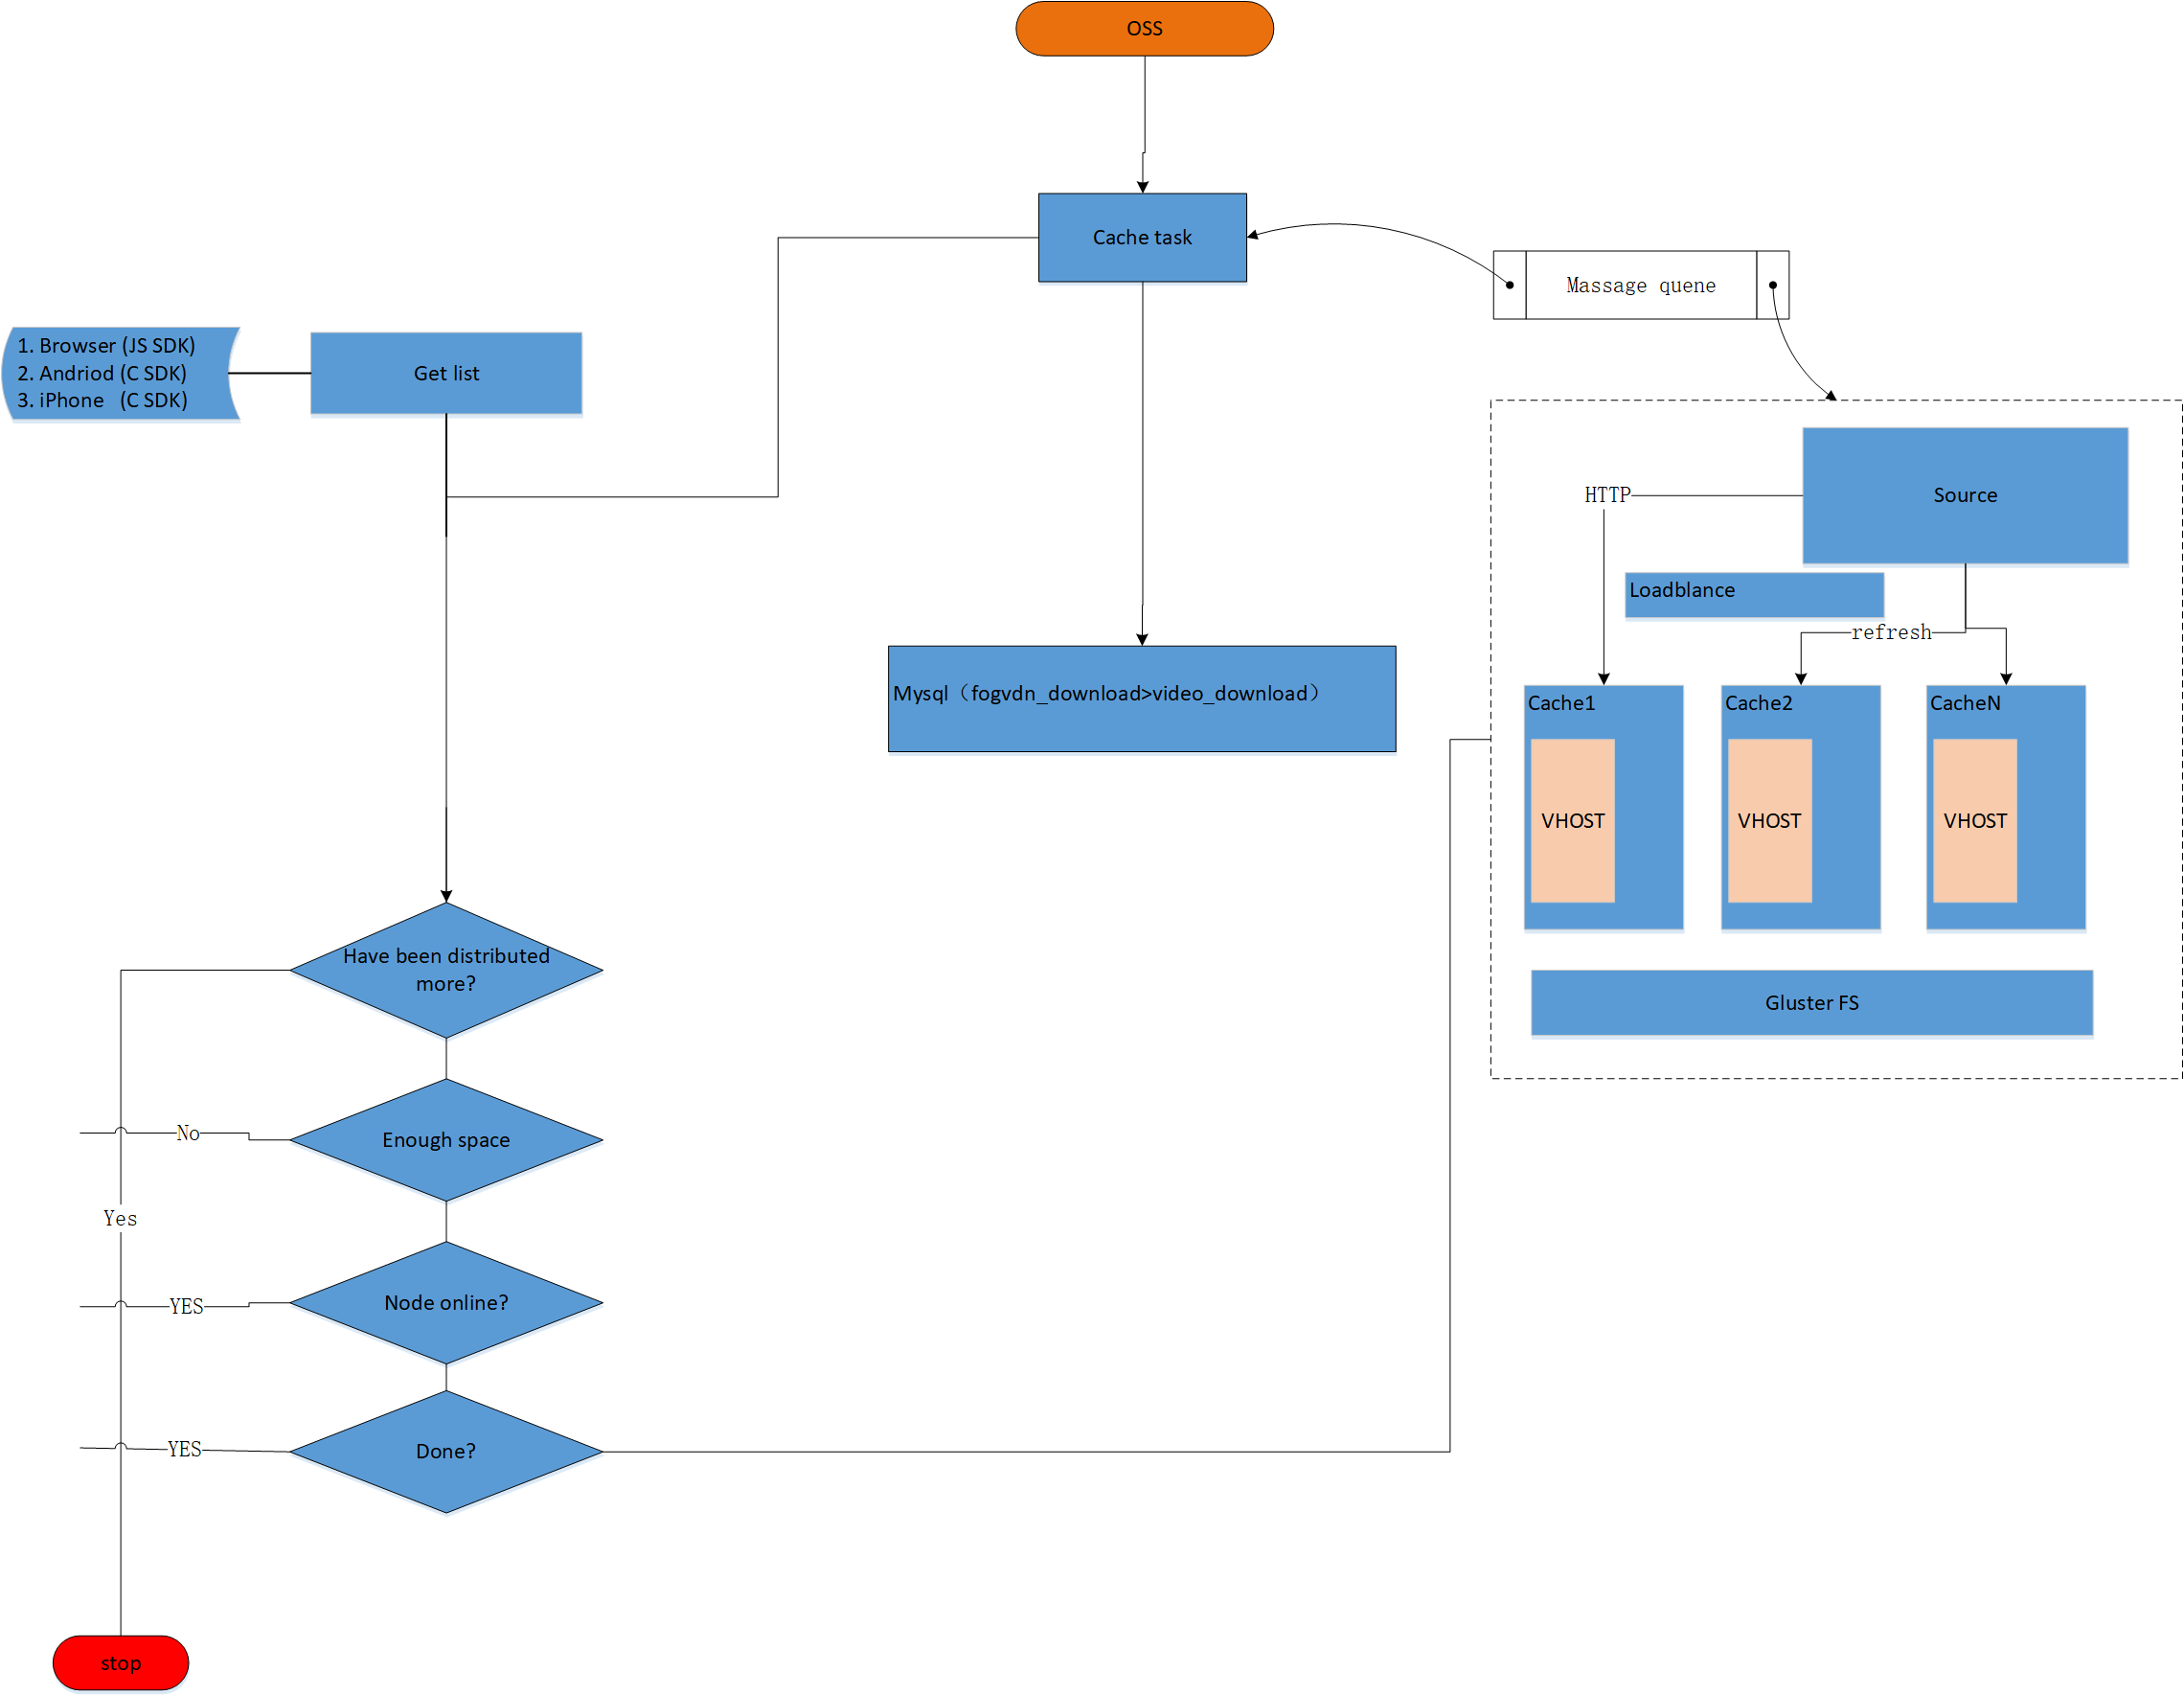
\includegraphics[width=\textwidth]{fig_11.png}
    \caption{Architecture of the "Content Manage System"(CMS)}
 \label{fig_11}
\end{figure}
\begin{figure}[htbp]
\centering
	  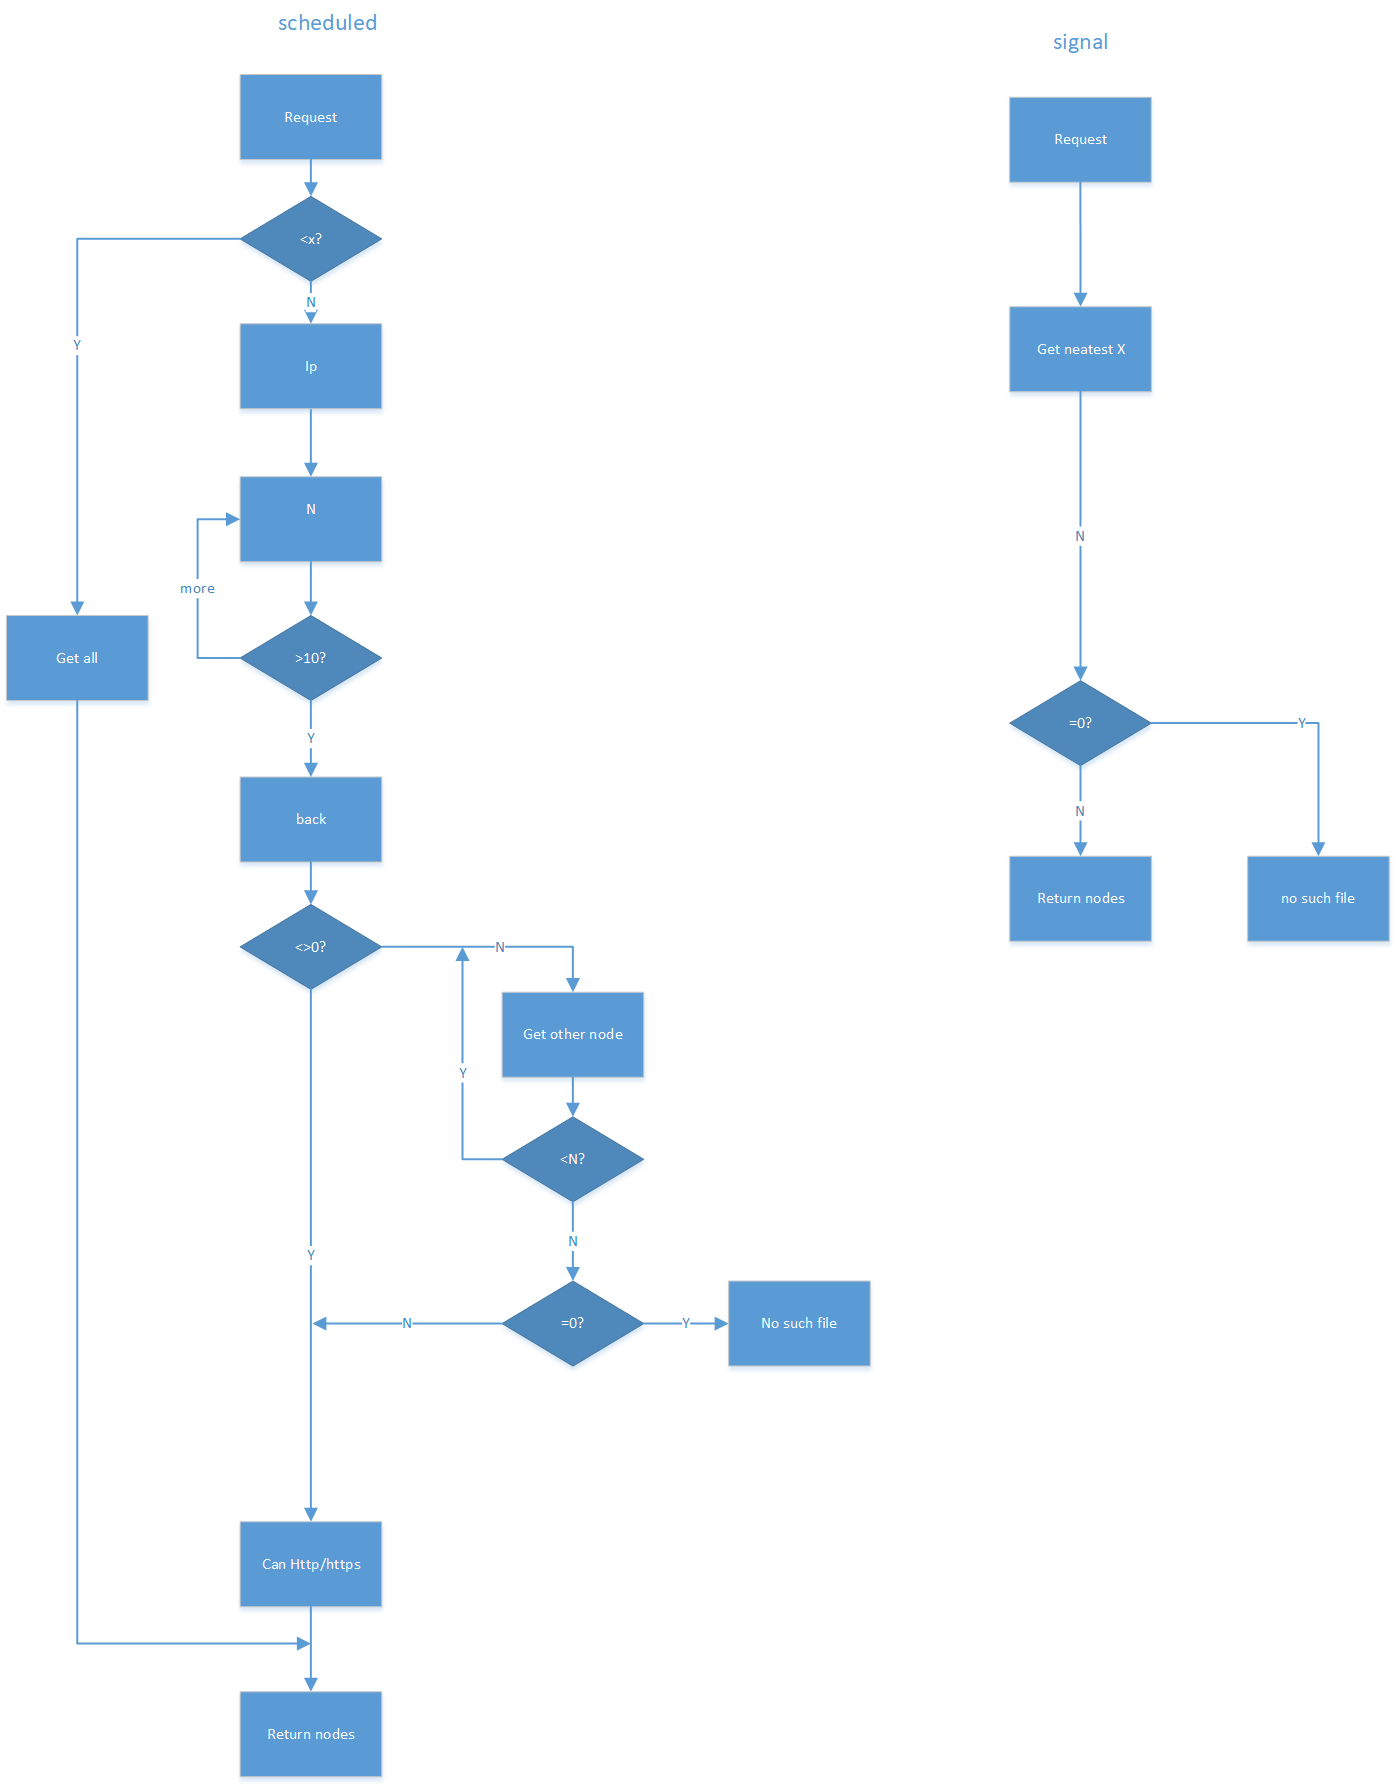
\includegraphics[width=\textwidth]{fig_12.png}
    \caption{Architecture of the "Node Manage System"(NMS)}
 \label{fig_12}
\end{figure}
\begin{figure}[htbp]
\centering
	  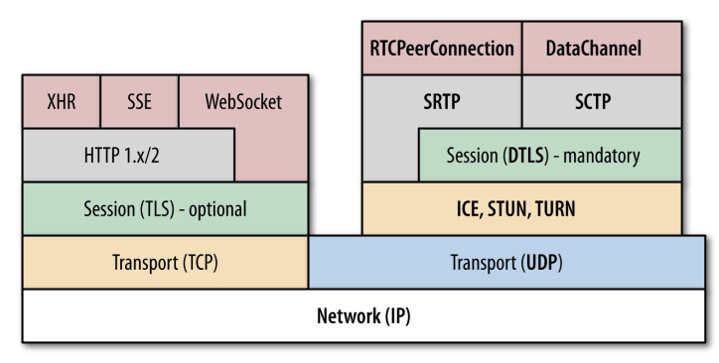
\includegraphics[width=\textwidth]{fig_18.png}
    \caption{WebRTC Stack}
 \label{fig_18}
\end{figure}

\begin{figure}[htbp]
\centering
	  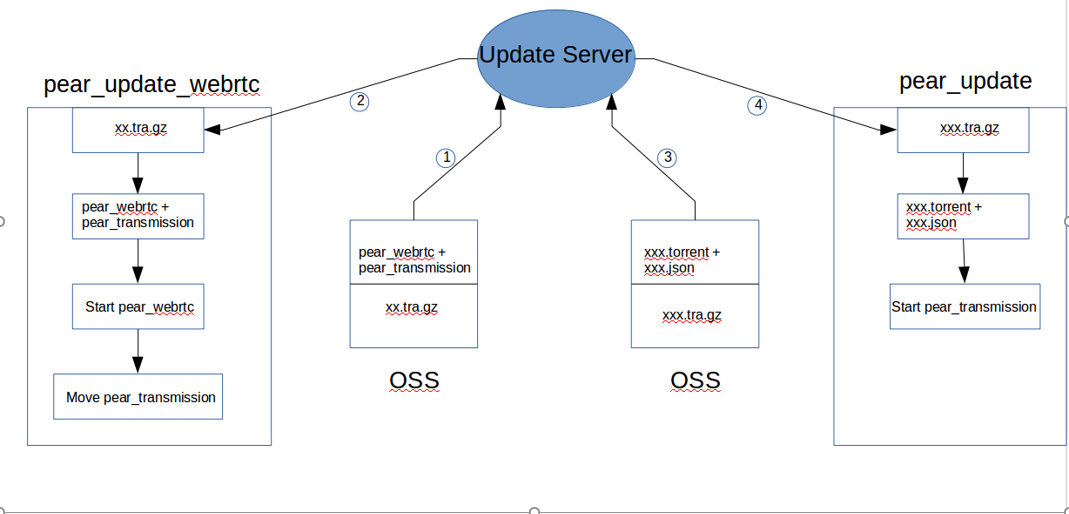
\includegraphics[width=\textwidth]{fig_19.png}
    \caption{Transmission combine WebRTC}
 \label{fig_19}
\end{figure}

\begin{figure}[htbp]
\centering
	  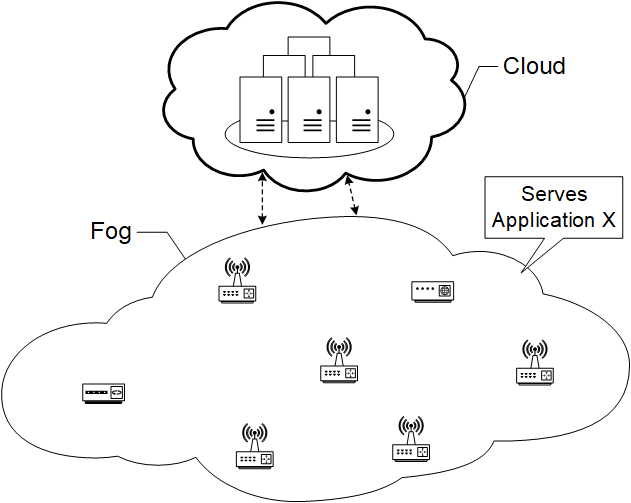
\includegraphics[width=\textwidth]{fig_27.png}
    \caption{Simple architecture of the "Fog as a Service"(FaaS)}
 \label{fig_27}
\end{figure}

  \chapter{User Test Report }
\label{chap:appC}
\begin{figure}[htbp]
\centering
	  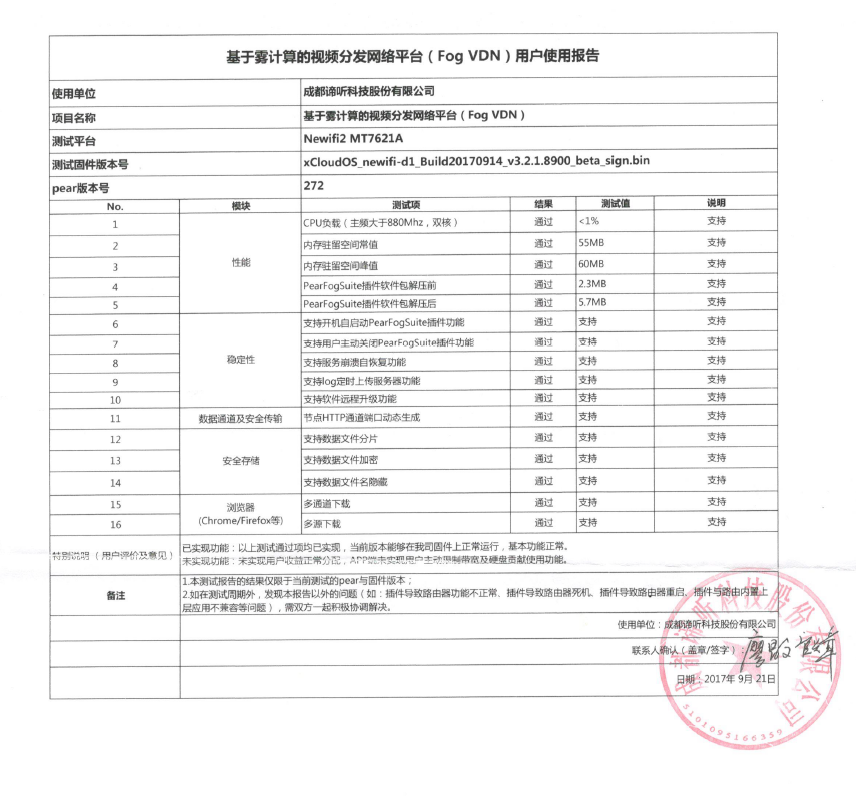
\includegraphics[width=\textwidth]{fig_15.png}
    \caption{Test Report from Newifi}
 \label{fig_15}
\end{figure}

  \chapter{User Incentive}
\label{chap:appD}
\begin{figure}[htbp]
\centering
	  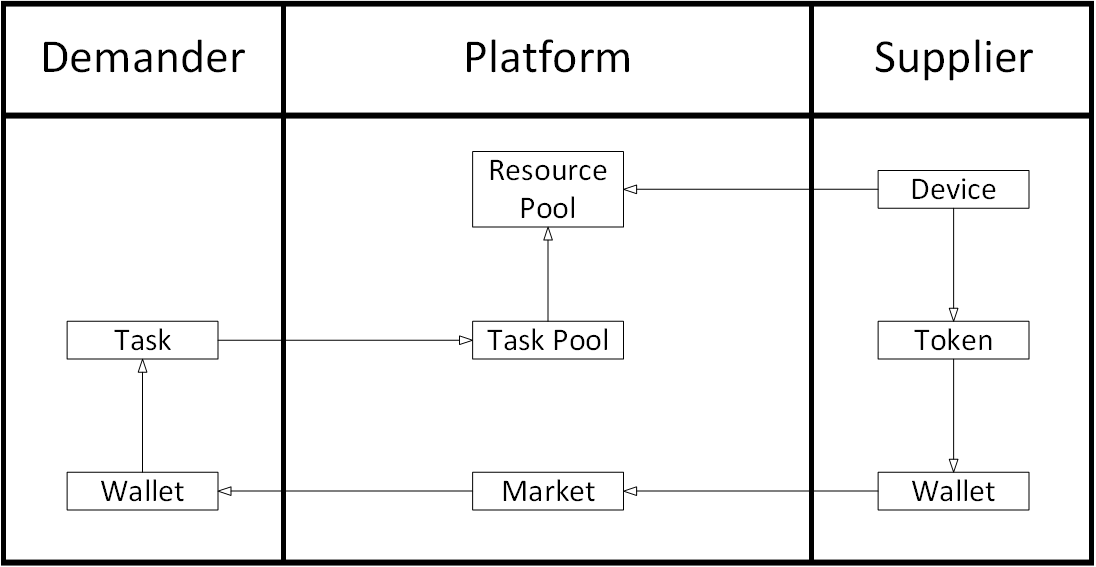
\includegraphics[width=\textwidth]{fig_16.png}
    \caption{Ecosystem Model}
 \label{fig_16}
\end{figure}

  \chapter{System Interface and Node Information}
\label{chap:appE}

\begin{figure}[htbp]
\centering
	  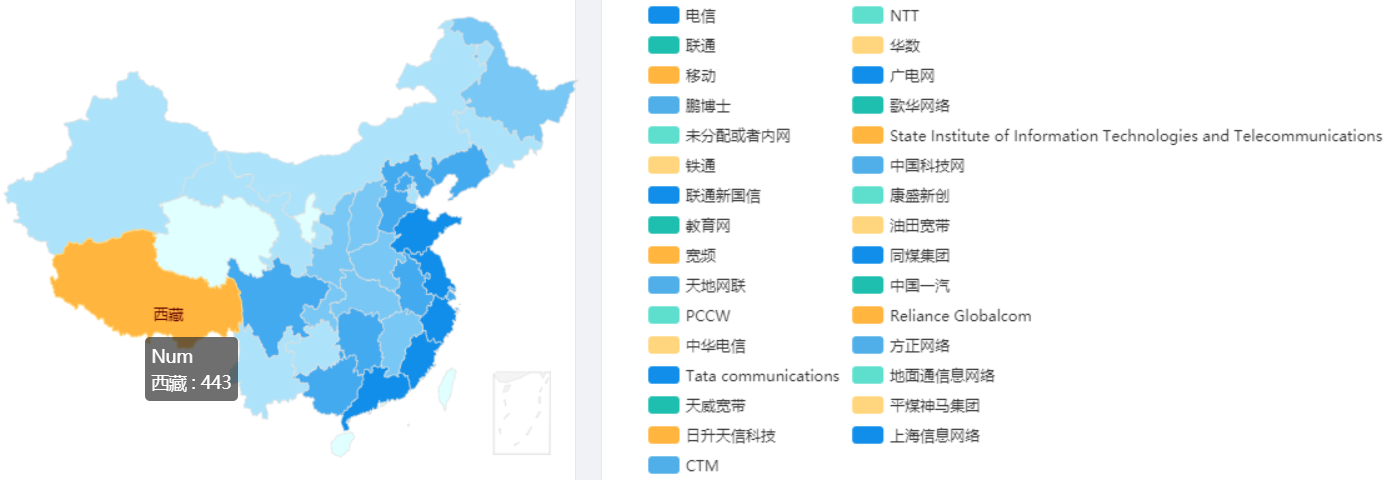
\includegraphics[width=\textwidth]{fig_24.png}
    \caption{Node distribution in China}
 \label{fig_24}
\end{figure}

\begin{figure}[htbp]
\centering
	  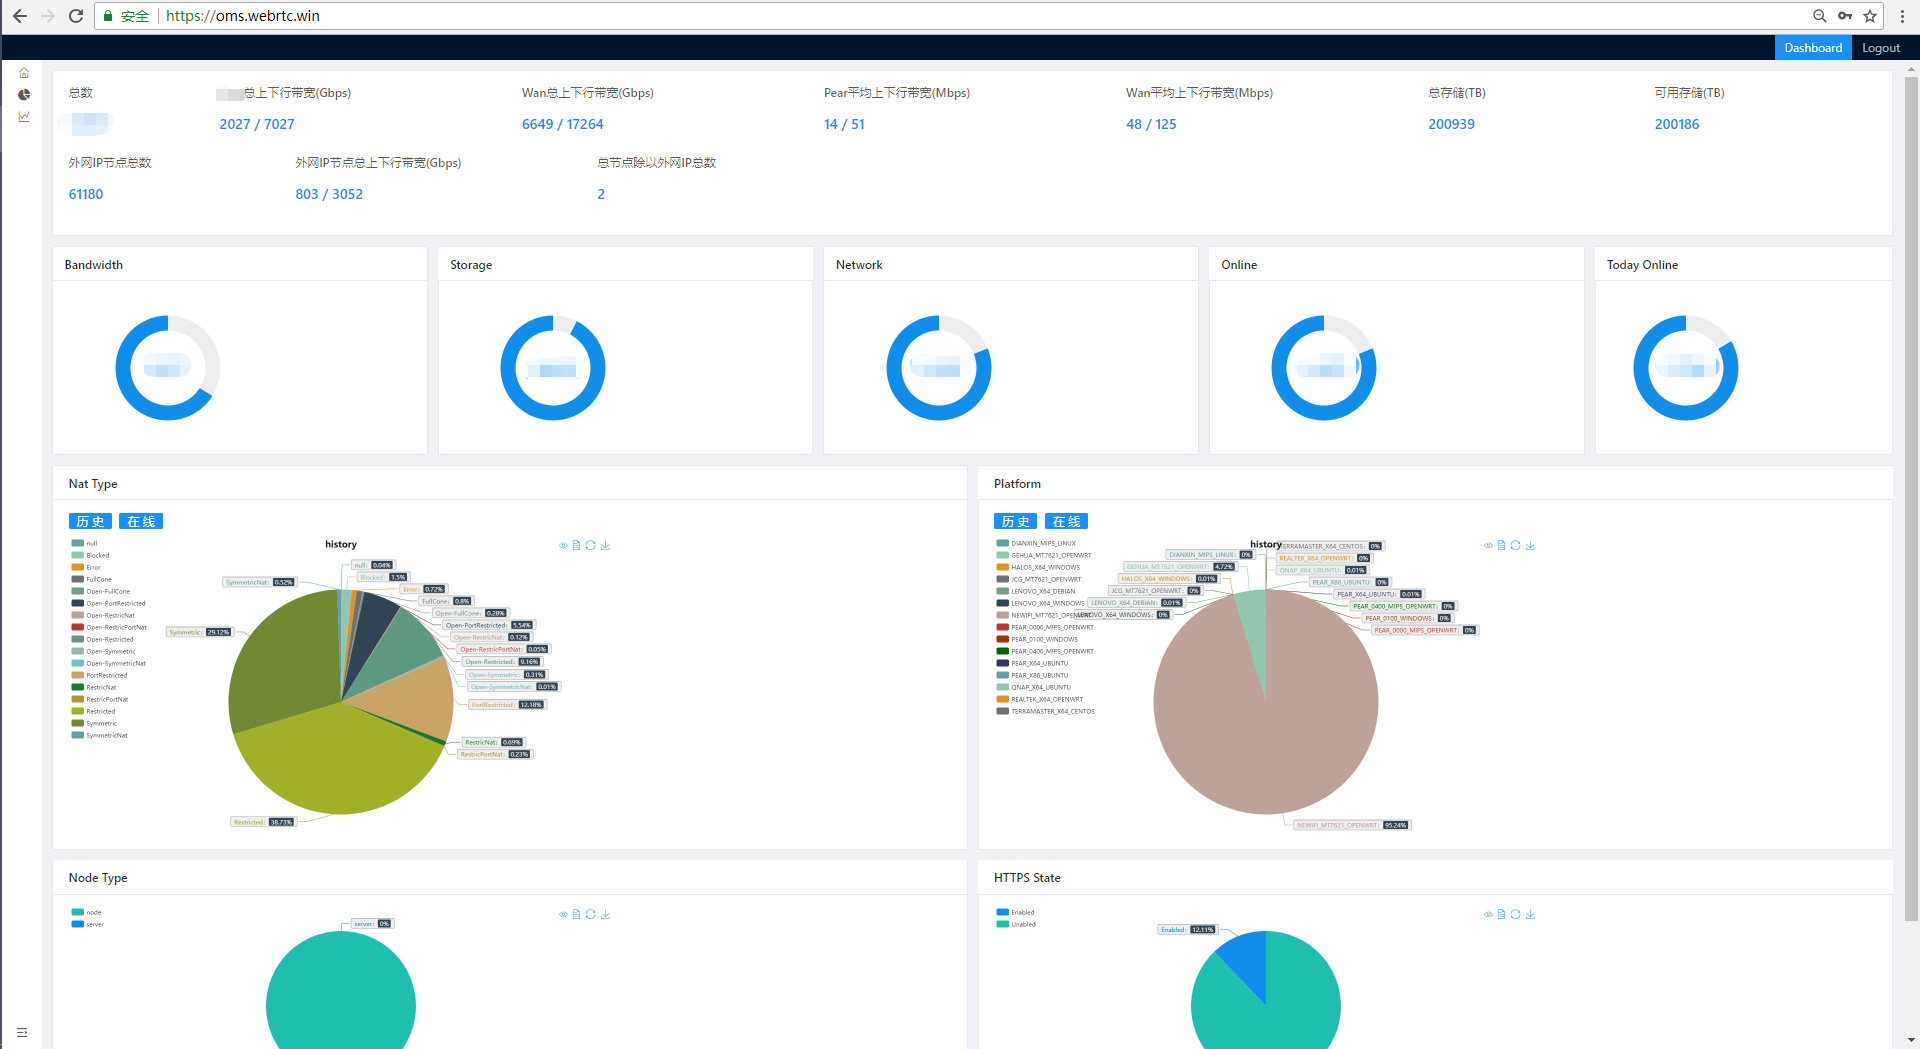
\includegraphics[width=\textwidth]{fig_29.png}
    \caption{OMS}
 \label{fig_29}
\end{figure}

\begin{figure}[htbp]
\centering
	  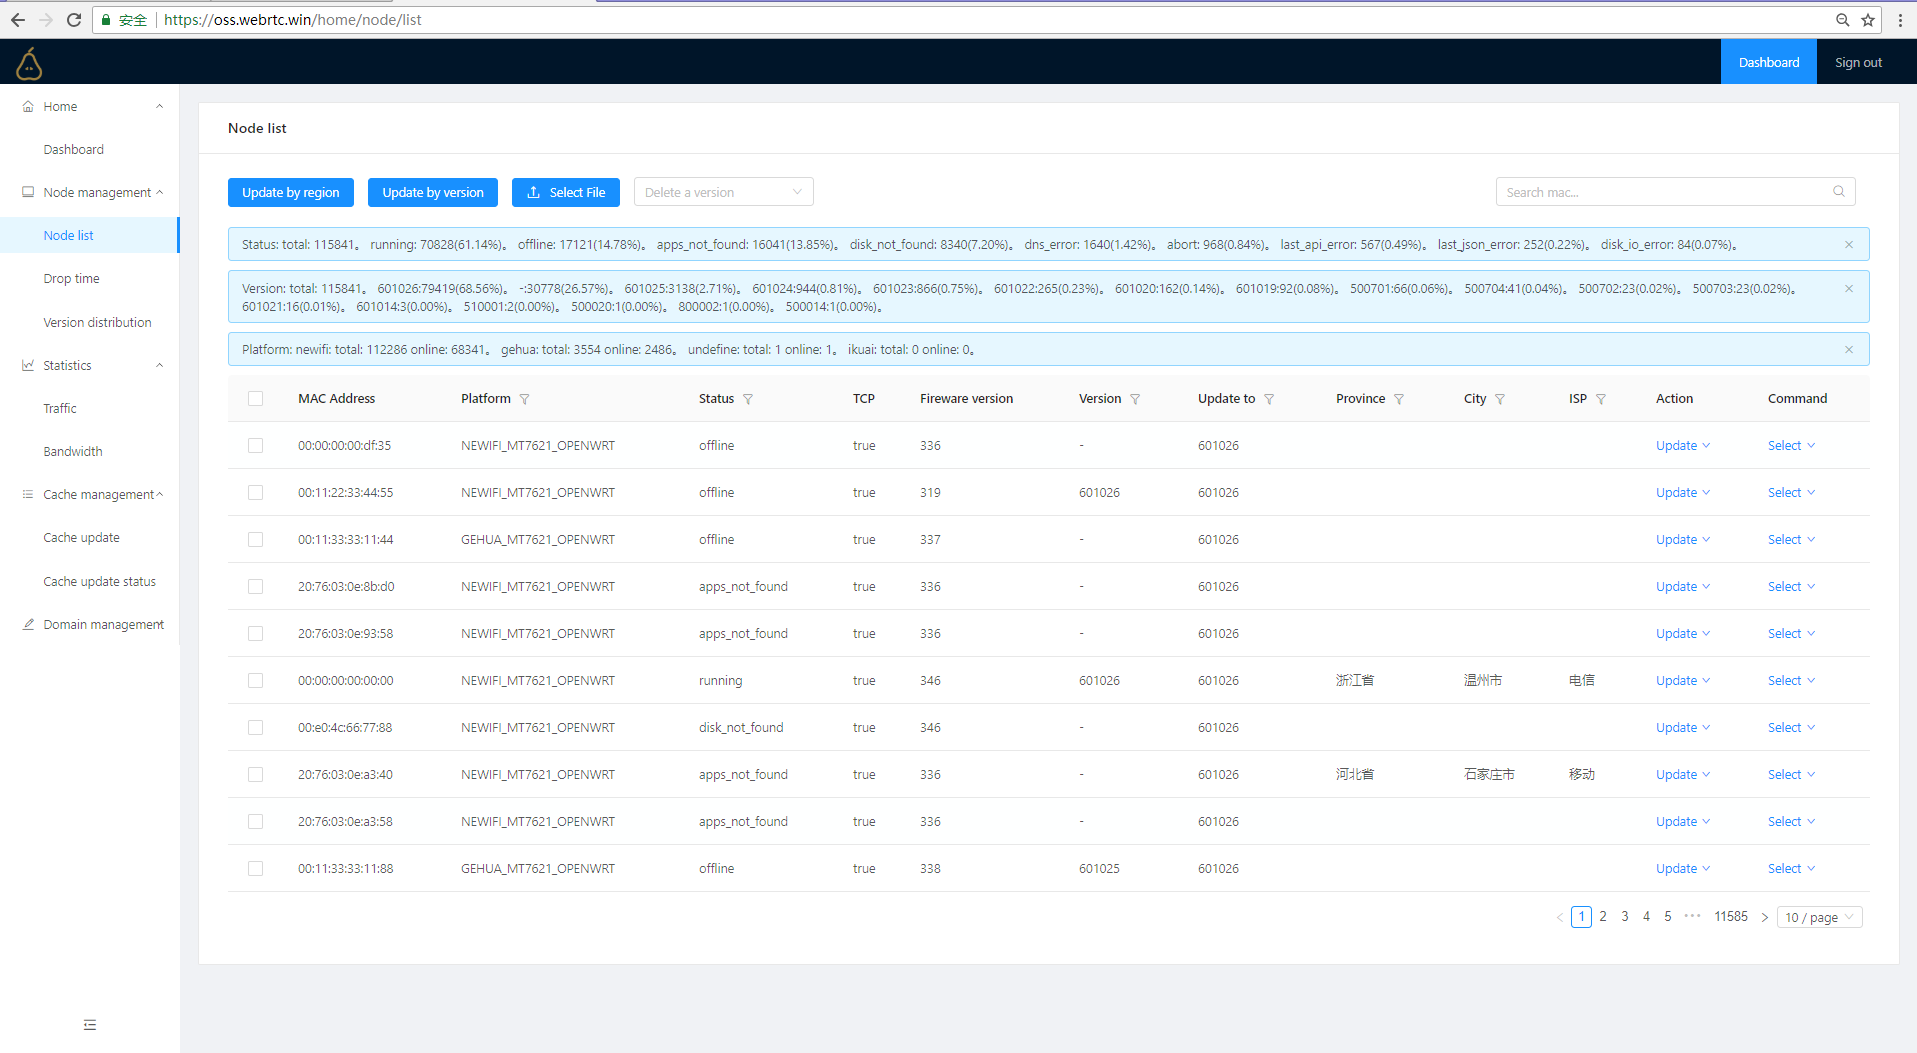
\includegraphics[width=\textwidth]{fig_30.png}
    \caption{NMS}
 \label{fig_30}
\end{figure}


\begin{figure}[htbp]
\centering
	  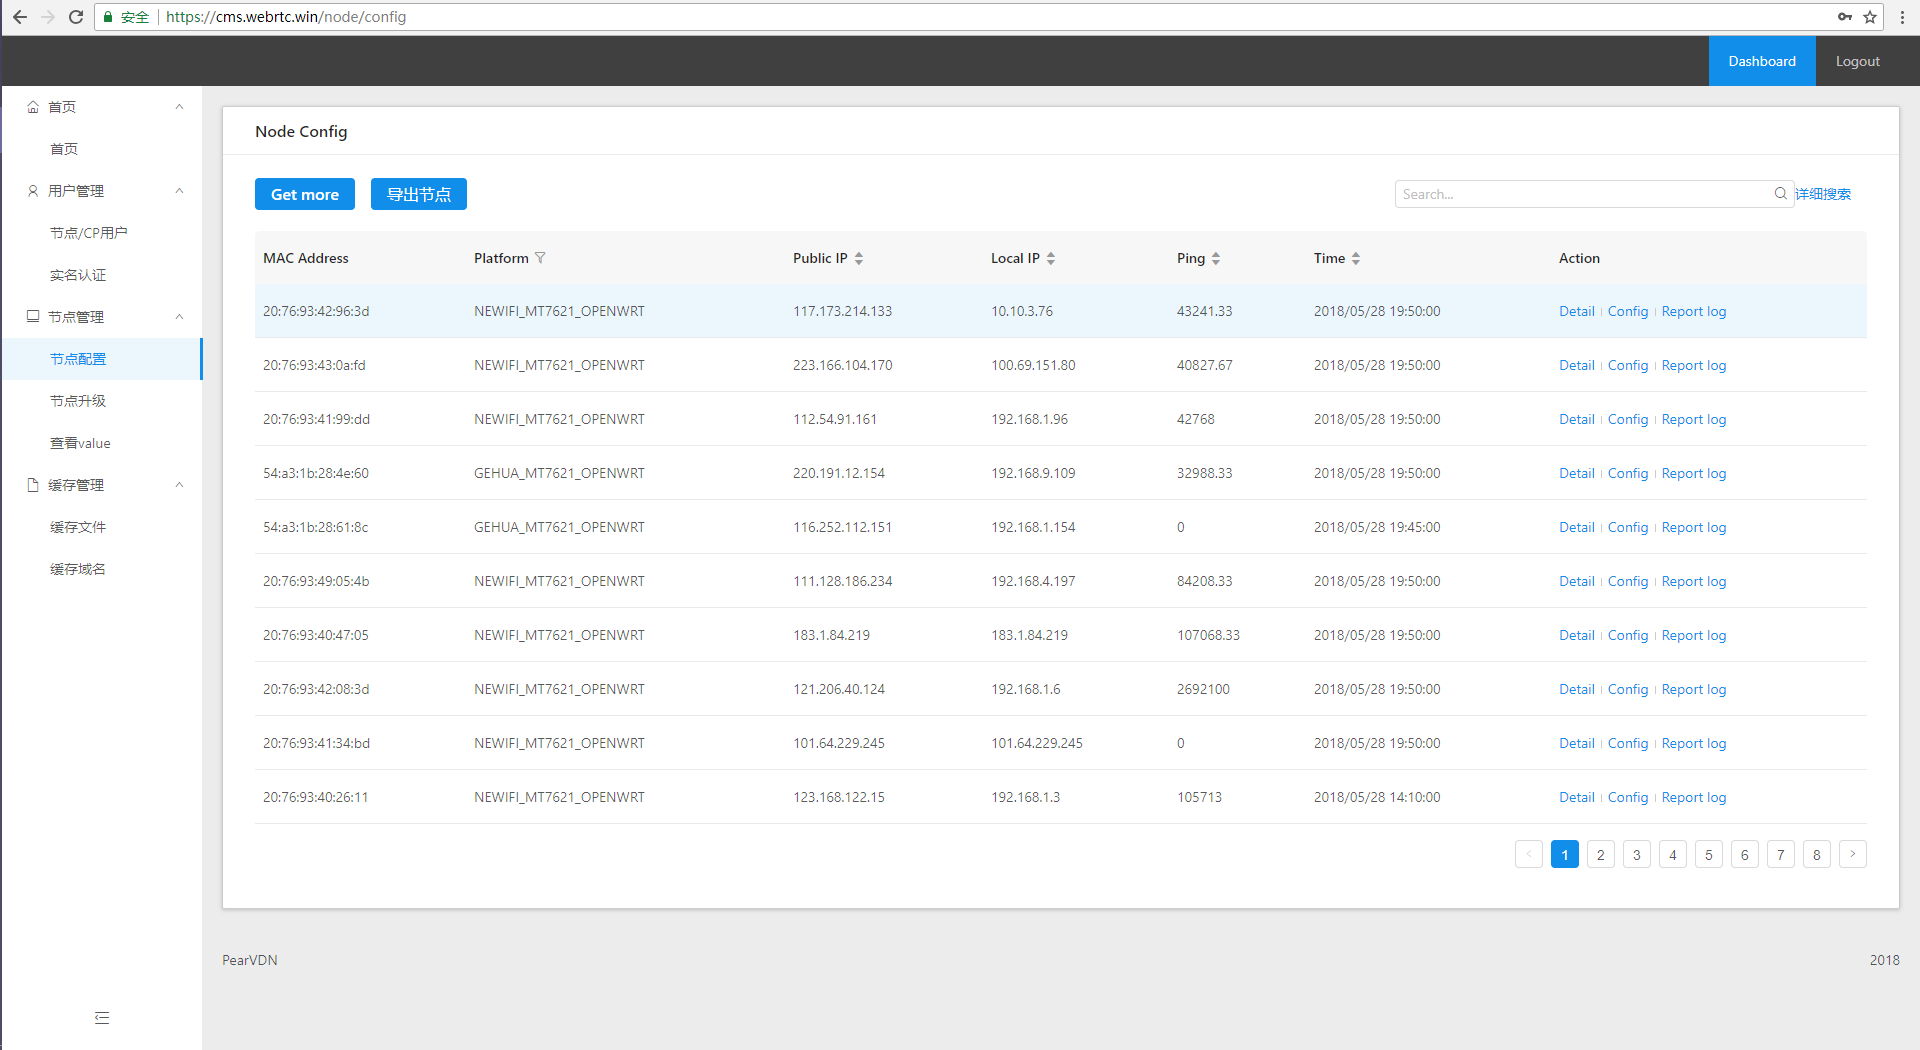
\includegraphics[width=\textwidth]{fig_31.png}
    \caption{CMS}
 \label{fig_31}
\end{figure}

\begin{figure}[htbp]
\centering
	  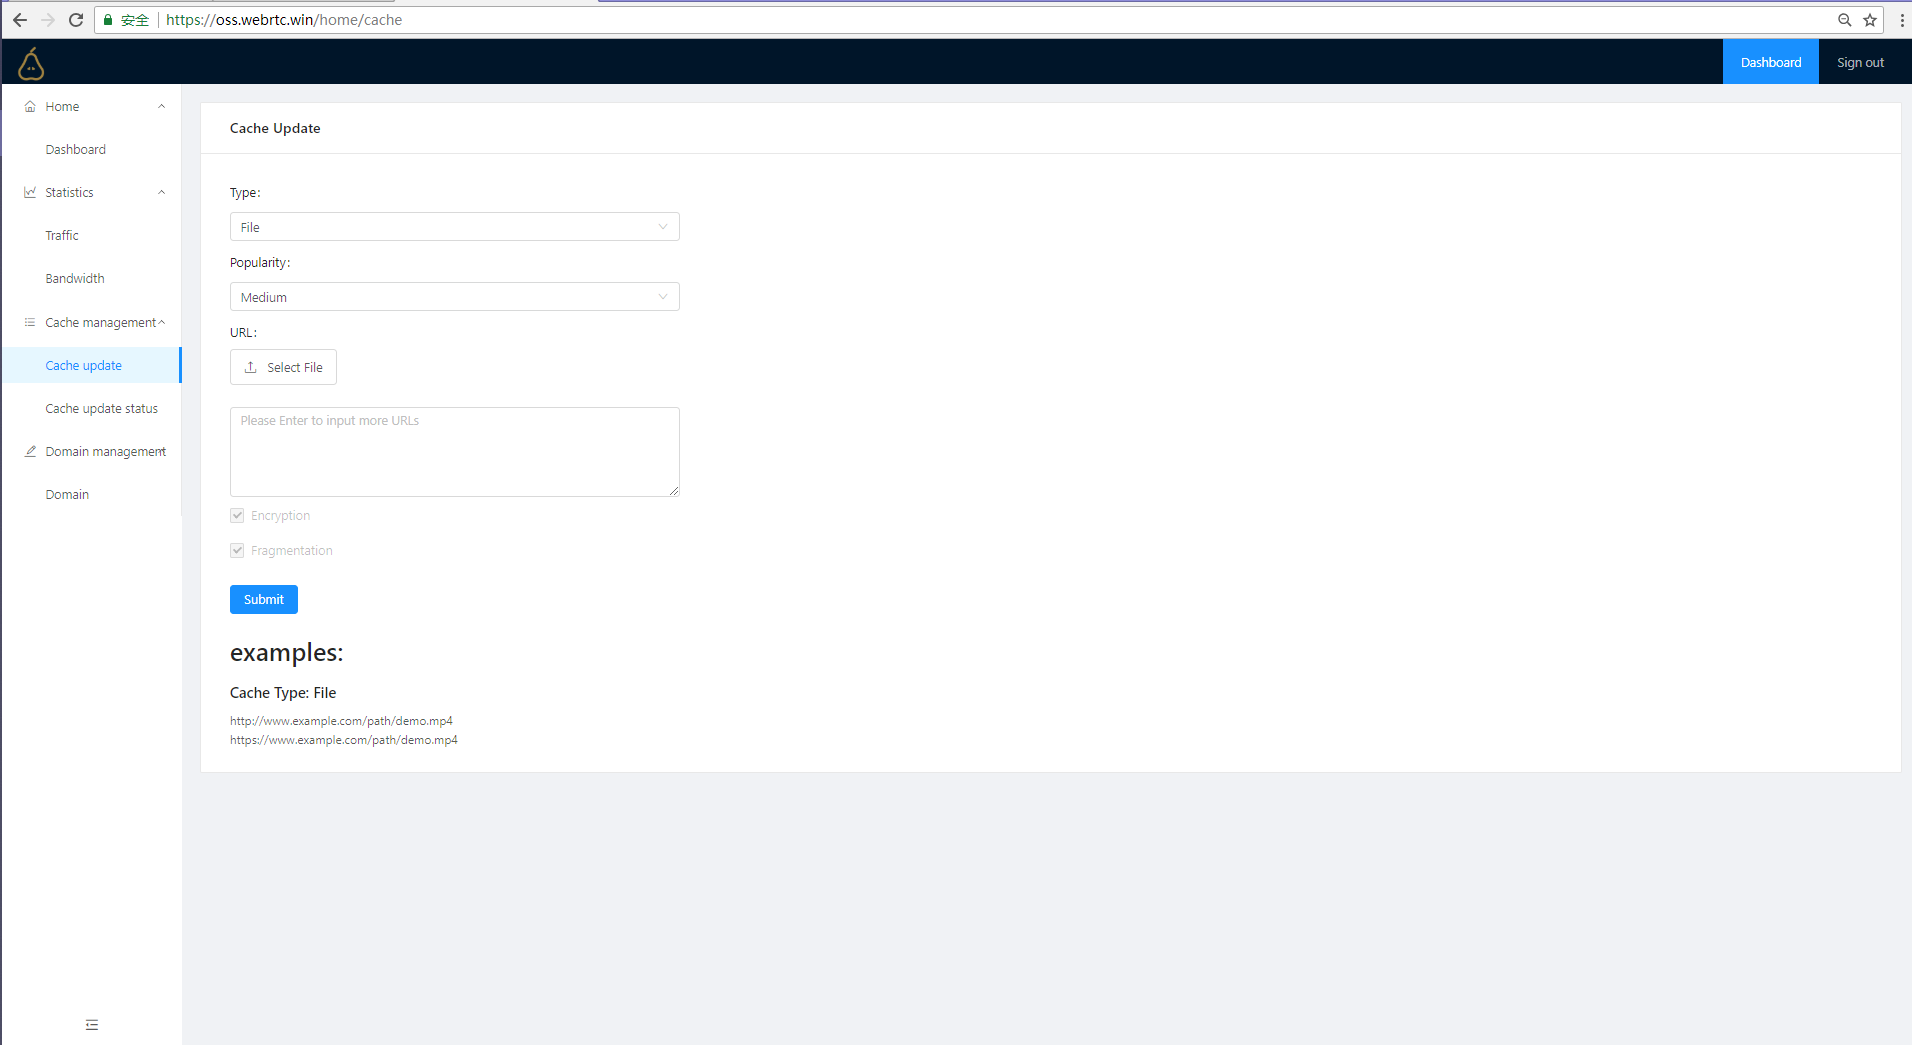
\includegraphics[width=\textwidth]{fig_32.png}
    \caption{OSS}
 \label{fig_32}
\end{figure}

\begin{figure}[htbp]
\centering
	  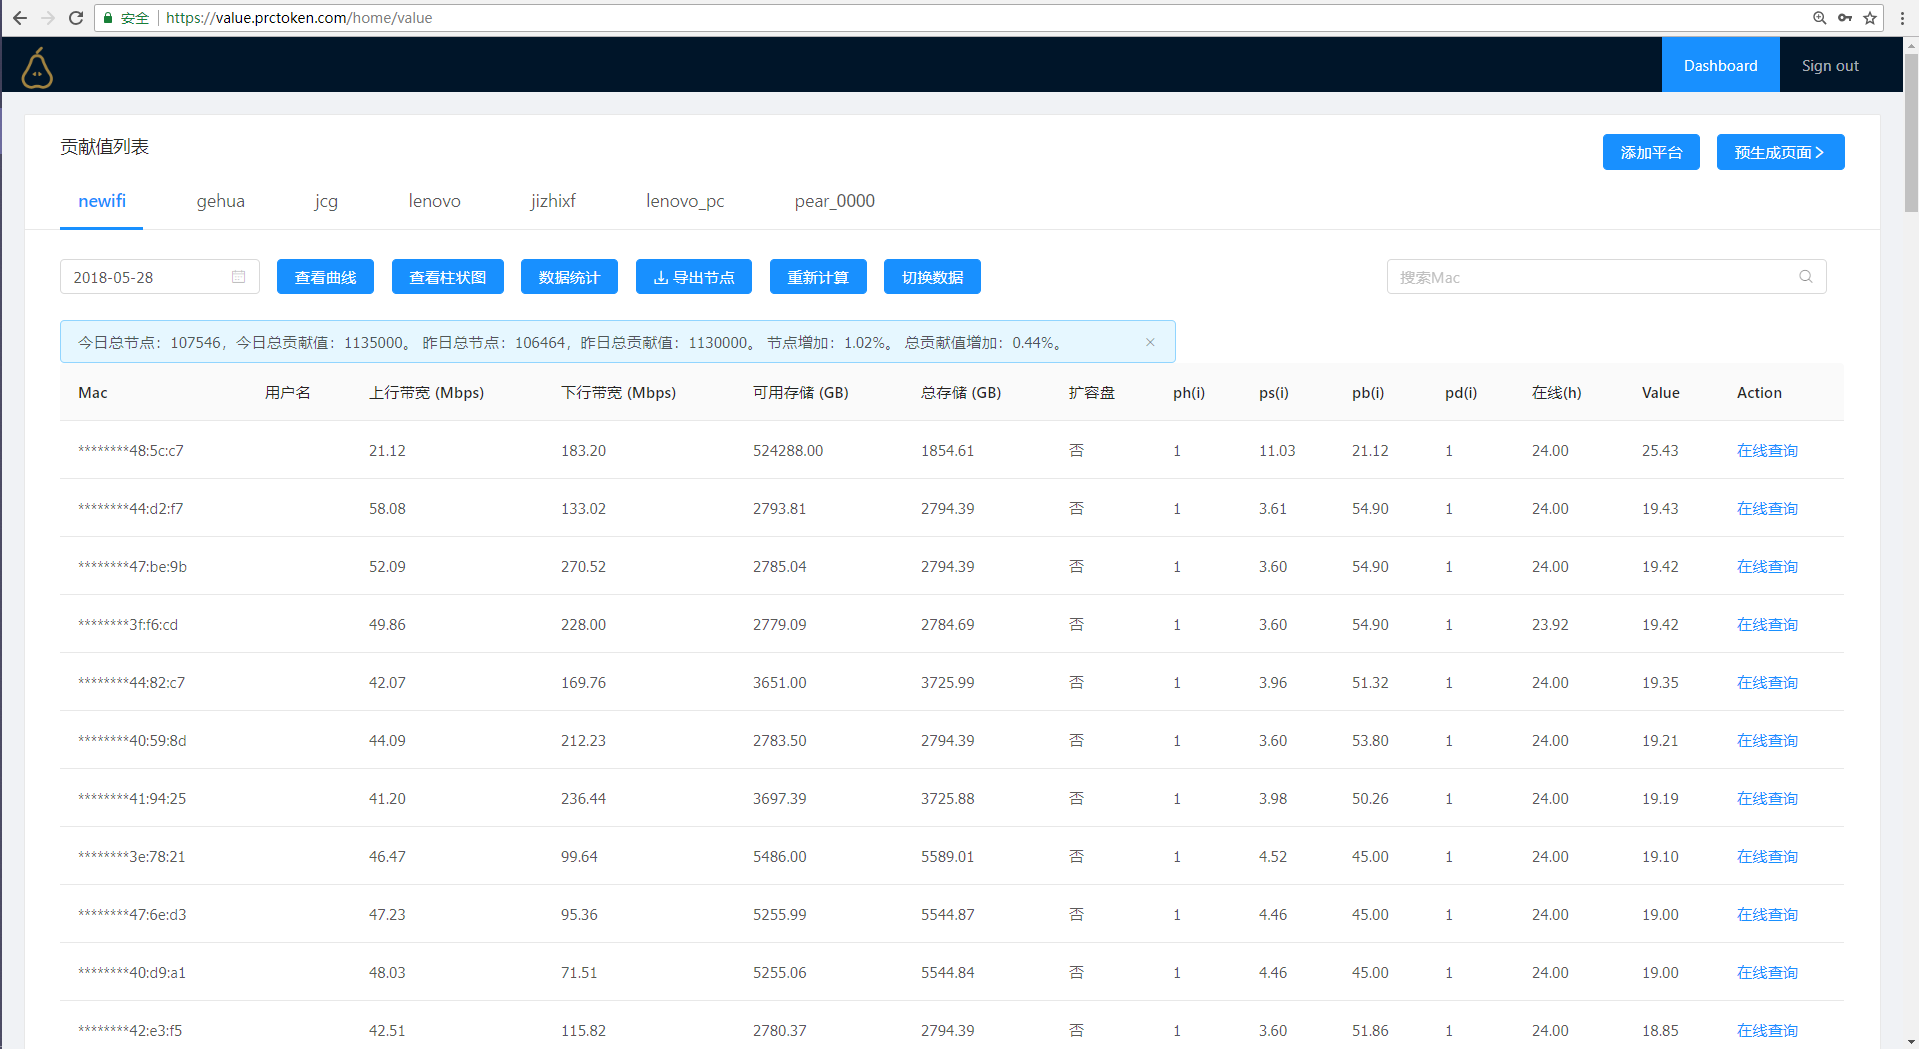
\includegraphics[width=\textwidth]{fig_33.png}
    \caption{PRC}
 \label{fig_33}
\end{figure}

\begin{figure}[htbp]
\centering
	  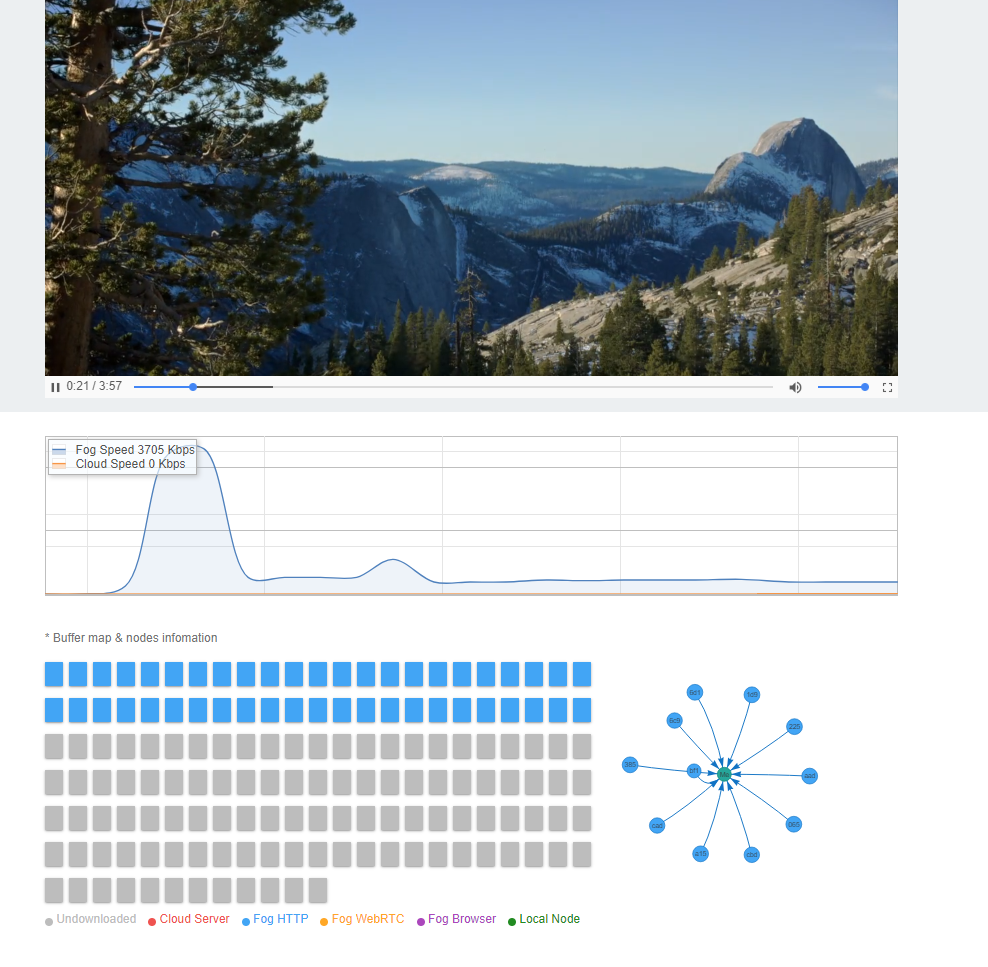
\includegraphics[width=\textwidth]{fig_34.png}
    \caption{Fog Player}
 \label{fig_34}
\end{figure}

\begin{figure}[htbp]
\centering
	  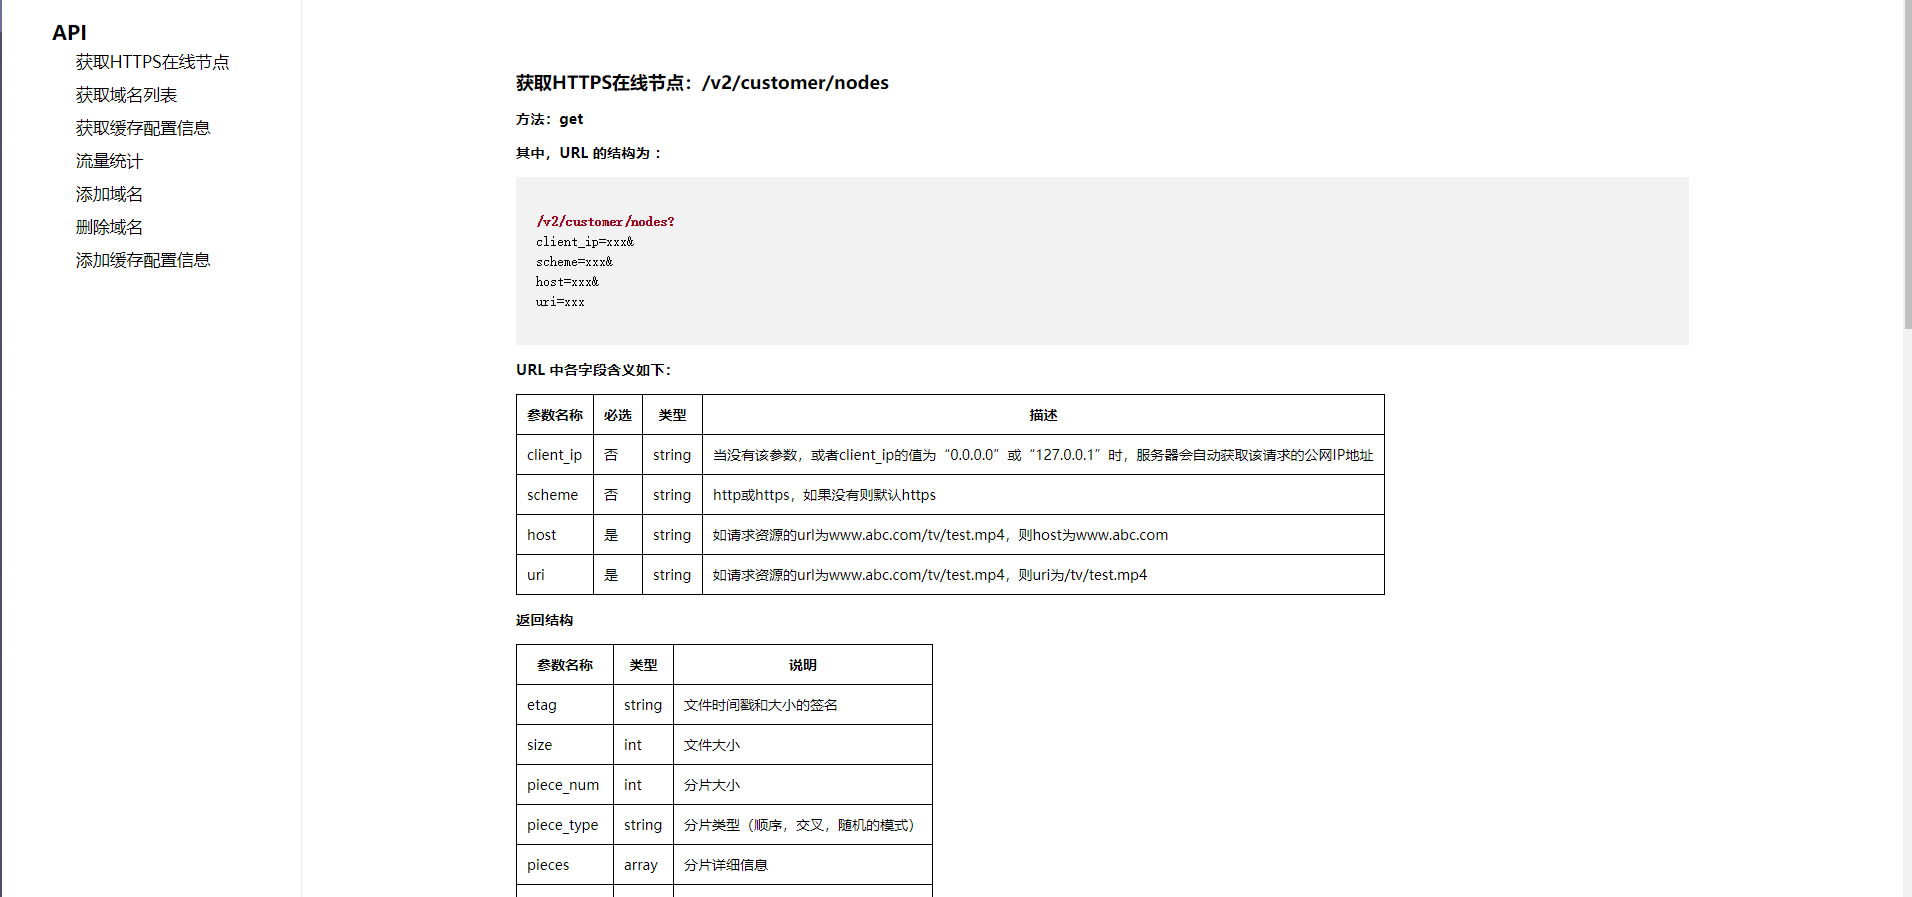
\includegraphics[width=\textwidth]{fig_35.png}
    \caption{Fog API}
 \label{fig_35}
\end{figure}

 \end{appendix}

%  \begin{thanks}
This thesis is the result of many years of study whereby I have been accompanied and supported by many people. It is a pleasure to convey my gratitude to all of them in my humble acknowledgement.

I want to give my sincerely thanks to my graduation designation supervisor Prof. Jingzhi Li for his earnest guidance and great help during my undergraduate study at SUSTC.

I would especially like to recognize my academic supervisors, Prof. Xianke Zhang and Prof. Jietai Yu, who have always given me encouragements and confidence in myself. They have played important roles in my decision to continue my education and inspired me for what I could achieve in the future. During the preparation of the thesis, we had many fruitful discussion. They have given me so many advises on the details of the thesis, including the tentative methods and writing techniques etc.

I am very grateful for all the encouragement I have received from my family and from a network of friends.  I would also like to thank my wonderful committee of professors. The committee members Prof. Xianke Zhang, Prof. Jingzhi Li, Prof. Anyue Chen, Prof. Xuejun Jiang and Prof. Linlin Su, who have contributed to the completion of this thesis through their guidance and exceptional teaching, which have helped me get through my education this far.  


Finally, I'd like to say thanks to all my teachers in SUSTC, especially teachers in the Department of Financial Mathematics for providing a stimulating environment. I am very grateful for all the encouragement I have received from my family and from a network of friends. 



\vskip 18pt

\begin{flushright}

Wenchao Zhang

September,2014

\end{flushright}

\end{thanks}




\end{document}
